
\documentclass[10pt]{beamer}
\mode<presentation> {
\usetheme{CambridgeUS}
\usecolortheme{dolphin}
\setbeamertemplate{footline}[frame number] % To replace the footer line in all slides with a simple slide count uncomment this line
\setbeamertemplate{navigation symbols}{} % To remove the navigation symbols from the bottom of all slides uncomment this line
}

\usepackage{graphicx} % Allows including images
\usepackage{subcaption}
\usepackage{booktabs} % Allows the use of \toprule, \midrule and \bottomrule in tables
\usepackage{wrapfig}
\usepackage{graphicx}
\usepackage{grffile}
\usepackage{multirow}
\usepackage{lipsum}
\usepackage{xcolor}
\usepackage{amsmath,amssymb}
\usepackage{array}
%\usepackage{gensymb}
\usepackage{animate,media9}
\usepackage{caption}
\usepackage{appendixnumberbeamer} 
%\captionsetup{font=scriptsize,labelfont=scriptsize}
%\usepackage{parskip}
\usepackage[english]{babel}
\usefonttheme{serif}
\usepackage{tikz}
\usepackage{tkz-euclide}
\usetikzlibrary{shapes,arrows}
\usetikzlibrary{positioning,fit,calc}
\usepackage{algorithm}
\usepackage{algorithmic}
\usepackage{graphicx} % Allows including images
\usepackage{booktabs} % Allows the use of \toprule, \midrule and \bottomrule in tables
\usepackage{wrapfig}
\usepackage{multirow}
\usepackage{lipsum}
\usepackage{amsmath,amssymb}
\usepackage{array}
\usepackage{gensymb}
\usepackage{animate,media9,movie15}
%\usepackage{parskip}
\usepackage[english]{babel}
\usefonttheme{serif}

\tikzset{
	block/.style = {draw, fill=white, rectangle, minimum height=2em, minimum width=2em},
	tmp/.style  = {coordinate},
	sum/.style= {draw, fill=white, circle, node distance=1cm},
	input/.style = {coordinate},
	output/.style= {coordinate},
	pinstyle/.style = {pin edge={to-,thin,black}
	}
}

\DeclareMathOperator*{\argmax}{arg\,max}
\DeclareMathOperator*{\argmin}{arg\,min}
%----------------------------------------------------------------------------------------
%	TITLE PAGE
%----------------------------------------------------------------------------------------

\title[]{\textbf{Autonomous Aerial Navigation in an Obscurant-filled Environment}} % The short title appears at the bottom of every slide, the full title is only on the title page
%\subtitle{Guide : Prof. Ameer Mulla}
\author[]{Arvind Pandit } % Your name
\institute[] % Your institution as it will appear on the bottom of every slide, may be shorthand to save space
{
	Roll No: 211022001 \\
	Department of Electrical Engineering\\
	Indian Institute of Technology Dharwad\\ % Your institution for the title page
	
	
	\normalsize{Guide : Prof. Ameer Mulla}
	\medskip
%	\textit{john@smith.com} % Your email address
}
\date{\today} % Date, can be changed to a custom date
\titlegraphic{
\includegraphics[scale=0.07]{Indian_Institute_of_Technology_Dharwad_Logo.svg.png}}

\begin{document}


\begin{frame}
    \titlepage % Print the title page as the first slide
\end{frame}

\begin{frame}
    \frametitle{Overview} % Table of contents slide, comment this block out to remove it
    \tableofcontents % Throughout your presentation, if you choose to use \section{} and \subsection{} commands, these will automatically be printed on this slide as an overview of your presentation
\end{frame}

%----------------------------------------------------------------------------------------
%	PRESENTATION SLIDES
%----------------------------------------------------------------------------------------

%------------------------------------------------
%\section{First Section} % Sections can be created in order to organize your presentation into discrete blocks, all sections and subsections are automatically printed in the table of contents as an overview of the talk
%%------------------------------------------------
%
%\subsection{Subsection Example} % A subsection can be created just before a set of slides with  a common theme to further break down your presentation into chunks
\section*{}
\begin{frame}{}
    \huge{\centerline{\textcolor{blue}{\textbf{1. Introduction}}}}
\end{frame}


\section{Introduction}
\subsection*{Motivation}
\begin{frame}{Motivation and Objective}
    \begin{block}{Motivation}
        \begin{itemize}
            \item WTC attack 2001(2,977 people), AMRI hospital fire 2011(90 people), Mundka fire 2022(27-people)
            \item Drone in the exploration task
            \item Deploy a drone for victim detection
            \item Fire dynamics and materials - Fire research group(IIT Dharwad)
            \item We are working on Autonomous Aerial navigation and human detection
        \end{itemize}
    \end{block}

    \pause \begin{block}{Objective}
        \begin{itemize}
            \item Autonomously navigates through the structure fire
            \item Localization and obstacle avoidance
            \item Detect human victims
            \item Transmit the position to base station
            \item Return path planning
        \end{itemize}
    \end{block}
\end{frame}

\subsection*{System Architecture}
\begin{frame}{System Architecture}
    \begin{figure}[h!]
        \centering
        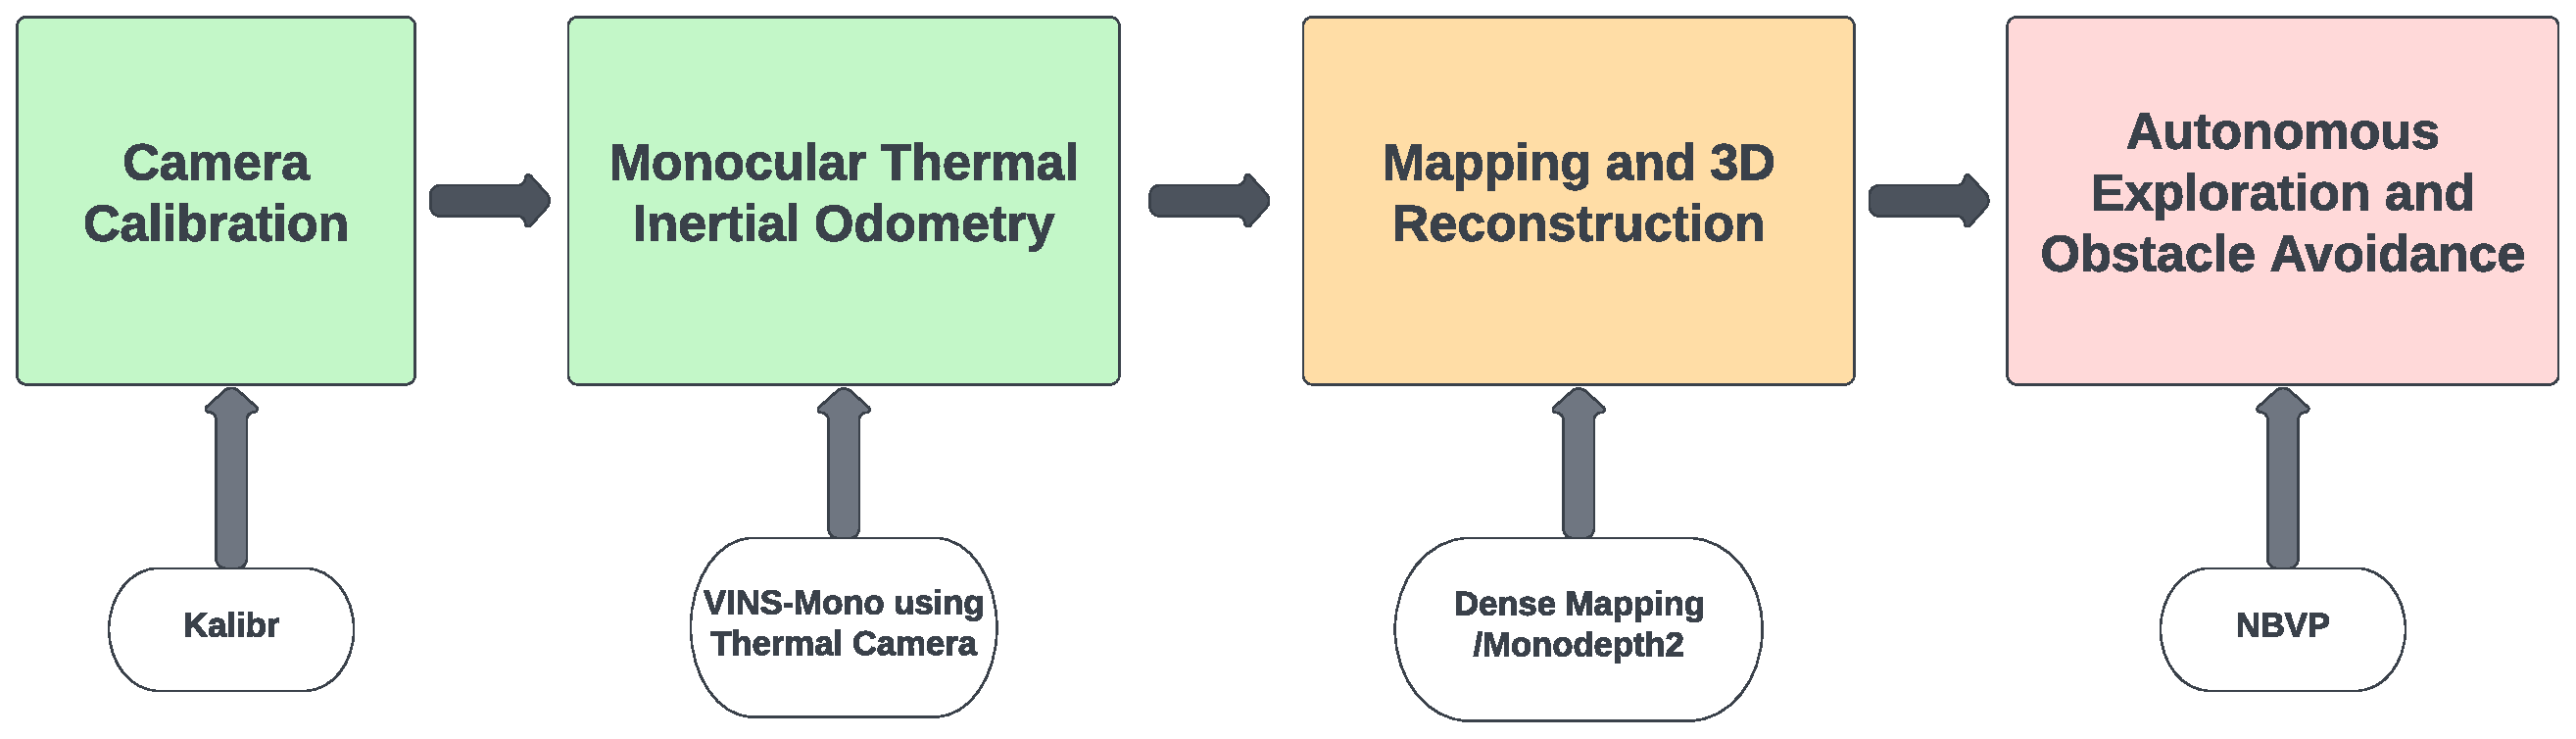
\includegraphics[scale=0.27]{TiHAN_Block_diagram.eps}
        \caption{System Pipeline}
        \label{Fig:System_Archi}
    \end{figure}
    \begin{itemize}
        \item \textbf{Camera Calibration :} Getting intrinsic camera parameters and extrinsic parameters of camera and IMU system.
        \item \textbf{Localization :} The 3D pose estimation of a quadcopter in a 3D space.
        \item \textbf{Mapping :} Dense mapping of an environment with obstacle information.
        \item \textbf{Exploration :} Frontier exploration and path planning.
    \end{itemize}{}
\end{frame}

\section*{}
\begin{frame}{}
    \huge{\centerline{\textcolor{blue}{\textbf{2. Monocular Visual Navigation }}}}
\end{frame}

\section{Monocular Visual Inertial Navigation System}
\subsection*{Camera Modeling and Calibration}
\begin{frame}{Camera Modeling and Calibration}
    \begin{figure}[!h]
        \centering
        \begin{subfigure}[b]{0.45\textwidth}
            \centering
            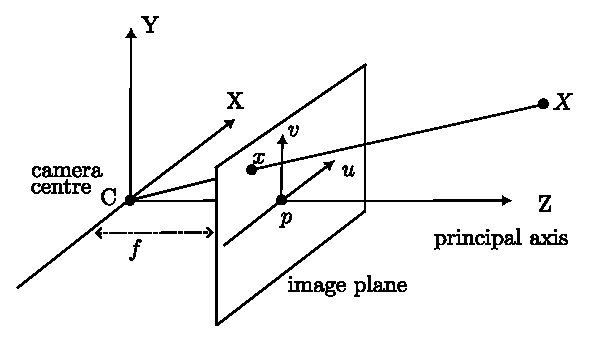
\includegraphics[scale=0.45]{cam_model.eps}
            \caption{Camera Coordinate Frames}
            \label{fig: Camera_coordinate}
        \end{subfigure}
        \hspace{1pt}
        \begin{subfigure}[b]{0.45\textwidth}
            \centering
            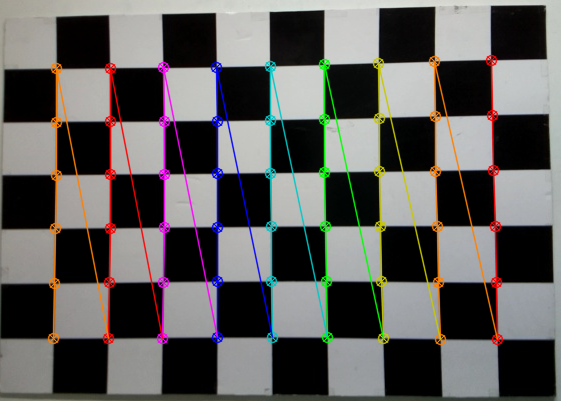
\includegraphics[scale=0.17]{CAm-cal.png}
            \caption{Camera Calibration}
            \label{fig: cam_cal}
        \end{subfigure}
        % \caption{Camera Model and Calibration}
        % \label{cam_mode_and_cal}
    \end{figure}
    \pause
    \begin{itemize}
        \item Homogeneous camera model
              \begin{equation}
                  \begin{bmatrix}
                      x^{\prime} \\
                      y^{\prime} \\
                      w^{\prime}
                  \end{bmatrix} =
                  \begin{bmatrix}
                      f_x & 0   & c_x \\
                      0   & f_y & c_y \\
                      0   & 0   & 1
                  \end{bmatrix}
                  \begin{bmatrix}
                      X \\
                      Y \\
                      Z
                  \end{bmatrix} or ~\mathbf{p}=\mathbf{K}\mathbf{X}
                  \label{eq:camera_model}
              \end{equation}
              where coordinates in the 2D image plane are given by $u=\frac{x^{\prime}}{w^{\prime}}~and~v=\frac{y^{\prime}}{w^{\prime}}$
        \item Zhang's camera calibration method with a chessboard is used \footnote{Z Zhang, A flexible new technique for camera calibration, 2000.}
    \end{itemize}
\end{frame}

\subsection*{Preliminaries}
\begin{frame}{Preliminaries}
    \begin{minipage}{0.47\textwidth}
        \begin{itemize}
            \item SfM is a reconstruction of structure using the different views of the camera.
        \end{itemize}
        \vspace{-0.2cm}
        \begin{figure}[h!]
            \centering
            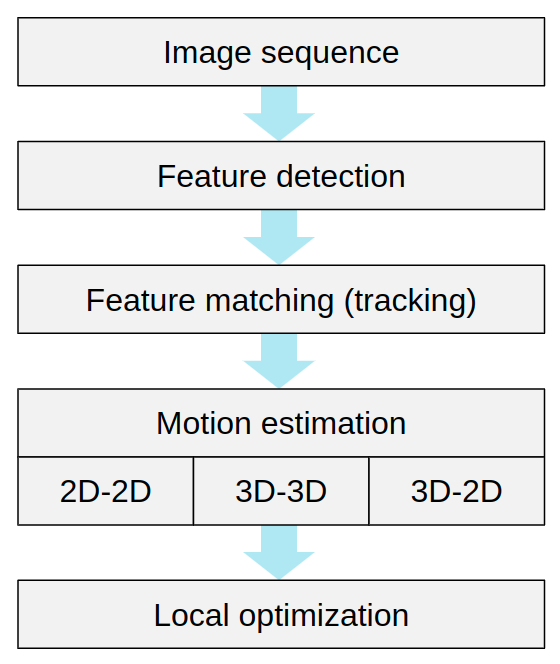
\includegraphics[scale=0.22]{Structure_from_motion_flow.png}
            \caption{Flow of Structure from Motion$^2$}
            \label{fig: Sfm_1}
        \end{figure}
    \end{minipage}
    \begin{minipage}{0.47\textwidth}
        \begin{itemize}
            \item An IMU gives data higher rate compare to camera.
            \item Position, velocity and orientation is estimated in this step.
            \item IMU residuals are calculated in this step.
        \end{itemize}
        \begin{figure}[h!]
            \centering
            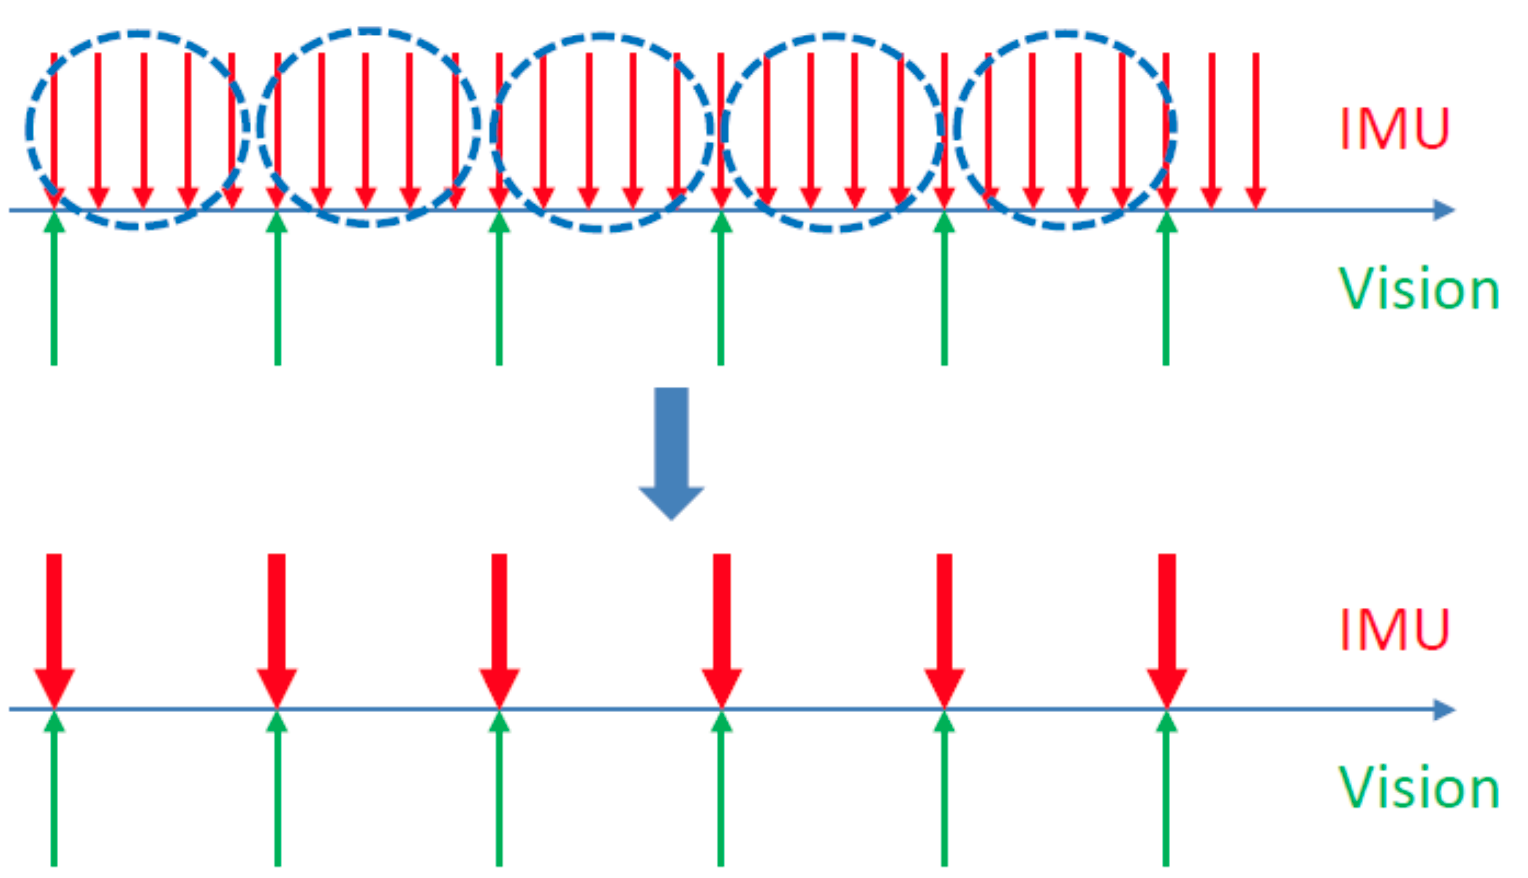
\includegraphics[scale=0.1]{Imu_preintegration.png}
            \caption{IMU Preintegration$^3$}
            \label{fig: imu_pre}
        \end{figure}
    \end{minipage}
    \footnote{D. Scaramuzza et al., Visual Odometry Tutorial, 2011.}
    \footnote{T Qin,et al. Vins-mono, 2018.}
\end{frame}

\subsection*{Visual Inertial Odomery}
\begin{frame}{Visual Inertial Odomery}
    \vspace{-0.2cm}
    \begin{figure}[h!]
        \centering
        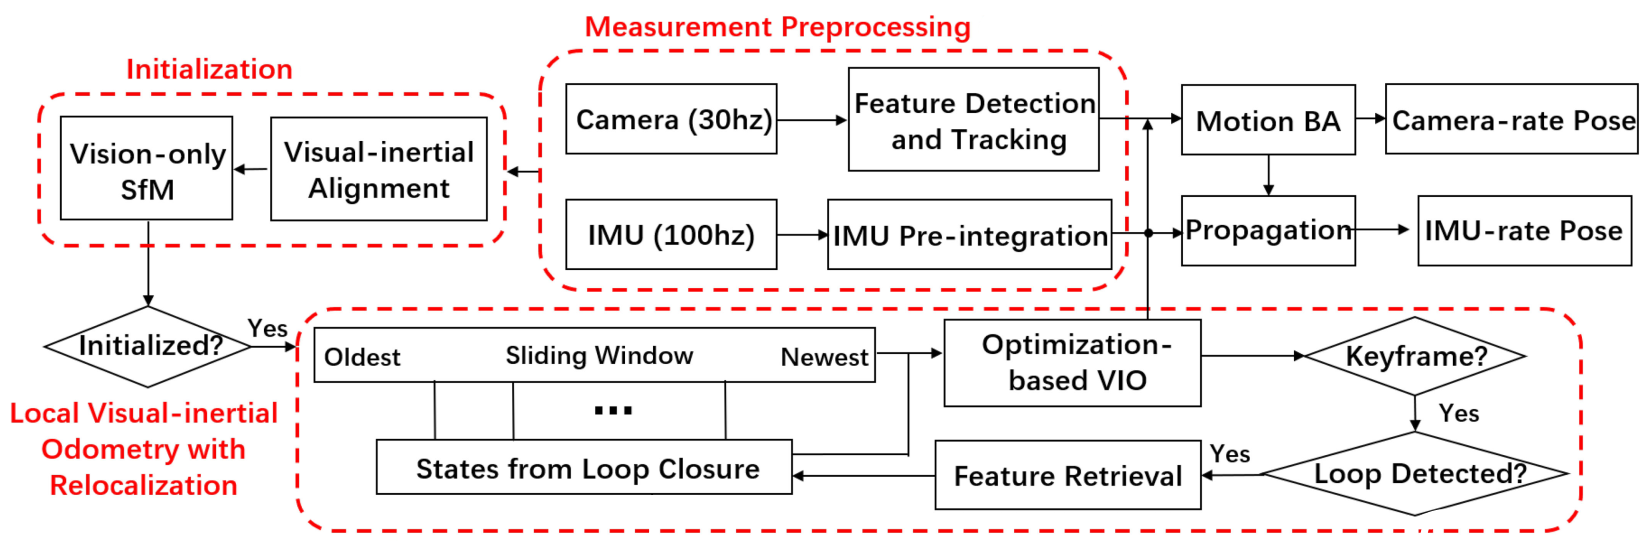
\includegraphics[scale=0.15]{VINS-mono-architecture.png}
        \caption{System Pipeline\footnote{T Qin,et al. Vins-mono, 2018.}}
        \label{Fig:System_Pipeline}
    \end{figure}
    \vspace{-0.6cm}
    \begin{itemize}
        \item \textbf{Initialization:} As the VIO is highly non-linear it needs a good initialization which is estimated in this section
              \pause
        \item \textbf{Measurement Preprocessing:} The visual and IMU measurement is preprocessed in this section and residuals of both are estimated
              \pause
        \item \textbf{Tightly Coupled Monocular VIO:} The main section where the IMU and visual measures are fused and the system is optimized with sliding window formulation
              \pause
        \item \textbf{Relocalization:} Relocalization reduce total drift in the estimated pose
    \end{itemize}
\end{frame}

% \subsection*{Tightly Coupled Monocular VIO}
% \begin{frame}{Tightly Coupled Monocular VIO}
%     \begin{description}
%         \item[1. Sliding window formulation]
%     \end{description}
%     \begin{itemize}
%         \item The full state vector
%               \begin{equation}
%                   \begin{split}
%                       \mathcal {X} &= \left[ \mathbf {x}_0,\,\mathbf {x}_{1},\, \ldots \,\mathbf {x}_{n},\, \mathbf {x}^b_c,\, \lambda _0,\,\lambda _{1},\, \ldots \,,\lambda _{m} \right] \\
%                       \mathbf {x}_k &= \left[ \mathbf {p}^w_{b_k},\,\mathbf {v}^w_{b_k},\,\mathbf {q}^w_{b_k}, \,\mathbf {b}_a, \,\mathbf {b}_g \right], k\in [0,n] \\
%                       \mathbf {x}^b_c &= \left[ \mathbf {p}^b_c,\,\mathbf {q}^b_{c} \right]
%                   \end{split}
%               \end{equation}

%               where \\
%               $\mathbf {x}_k$ - IMU state at the time that the kth image is captured\\
%               (It contains the position, velocity, and orientation of the IMU in the world frame, and acceleration bias and gyroscope bias in the IMU body frame.) \\
%               $\mathbf {x}^b_c$ - Transformation between IMU and camera frame from calibration.\\
%               $n$ - Total number of keyframes\\
%               $m$ - Total number of features in the sliding window \\
%               $\lambda_l$ - Inverse distance of the $l^{th}$ feature from its first observation
%     \end{itemize}{}
% \end{frame}
% \begin{frame}{}
%     \begin{description}
%         \item[2. Cost function]
%     \end{description}

%     \begin{itemize}
%         \item Bundle Adjustment cost function with IMU and camera residuals
%         \item The sum of prior and Mahalanobis norm of all measurements residuals are minimized to obtain a maximum posterior estimation \footnote{T Qin,et al. Vins-mono: A robust and versatile monocular visual-inertial state estimator, 2018.}
%               \begin{equation} \label{eq:1st_cost_func}
%                   \begin{split}
%                       \min _{\mathcal {X}} \left\lbrace \left\Vert \mathbf {r}_p - \mathbf {H}_p \mathcal {X} \right\Vert ^2 + \sum _{k \in \mathcal {B}} \left\Vert \mathbf {r}_{\mathcal {B}}(\hat{\mathbf {z}}^{b_k}_{b_{k+1}},\, \mathcal {X}) \right\Vert _{\mathbf {P}^{b_k}_{b_{k+1}}}^2 \right. \\
%                       \left. +\sum _{(l,j) \in \mathcal {C}} \rho (\left\Vert \mathbf {r}_{\mathcal {C}}(\hat{\mathbf {z}}^{c_j}_l, \, \mathcal {X}) \right\Vert _{\mathbf {P}^{c_j}_l}^2) \right\rbrace \end{split}
%               \end{equation}
%               where $\mathbf {r}_{\mathcal {B}}(\hat{\mathbf{z}}^{b_k}_{b_{k+1}},\, \mathcal {X})$ and $\mathbf {r}_{\mathcal {C}}(\hat{\mathbf {z}}^{c_j}_l,\, \mathcal {X})$ are residuals Huber norm is defined
%               \begin{equation}
%                   \rho (s)=\left\{\begin{array}{ll}s & s \leq 1\\ 2\sqrt{s}-1 & s > 1. \end{array}\right.
%               \end{equation}
%         \item $\lbrace\mathbf {r}_p,\,\mathbf {H}_p\rbrace$ is the prior information from marginalization.
%     \end{itemize}
% \end{frame}

\subsection*{3D Depth Estimation}
\begin{frame}{3D Depth Estimation}
    \begin{itemize}
        \item Standard Encoder-Decoder network with skip connnections is used for the depth estimation given a monocular RGB image.
    \end{itemize}
    \pause
    \begin{figure}[!ht]
        \centering
        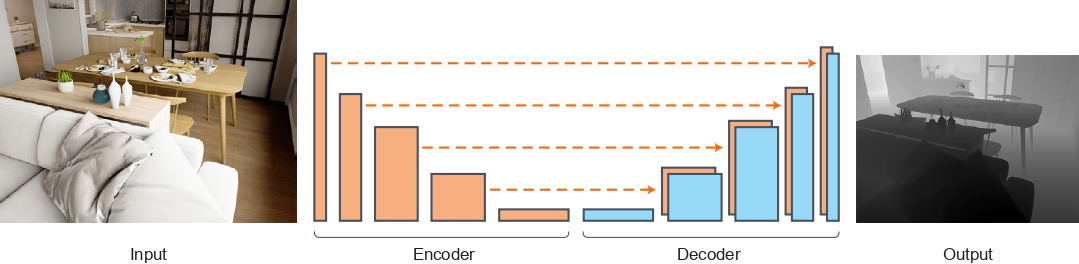
\includegraphics[scale=0.60]{monocular_depth.jpg}
        \caption{Network Architecture\footnote{Ibraheem, et al. High Quality Monocular Depth Estimation via Transfer Learning,2019}}
        \label{fig:net_archi}
    \end{figure}
    \pause
    \vspace{-0.5cm}
    \begin{itemize}
        \item Here DenseNet-169 network is used as encoder.
        \item Decoder uses same no. of output channels as truncated encoder's output.
        \item Series of bilinear upsampling block.
        \item Leaky ReLU as an activation function.
    \end{itemize}
\end{frame}

% \subsection*{Loss Fucntion}
% \begin{frame}{Loss Fucntion}
%     \begin{itemize}
%         \item The Loss function for the network is given by,\footnote{Ibraheem, et al. High Quality Monocular Depth Estimation via Transfer Learning,2019}
%               \begin{equation*}
%                   L(y,\hat{y}) = \lambda L_{depth}(y,\hat{y}) + L_{grad}(y,\hat{y}) + L_{SSIM}(y,\hat{y}).
%               \end{equation*}
%               \pause
%         \item $L_{depth}$ is the point-wise L1 loss defined on the depth values:
%               \begin{equation*}
%                   L_{depth}(y,\hat{y}) = \frac{1}{n} \sum_{p}^{n} \lvert y_p -\hat{y}_p \rvert.
%               \end{equation*}
%               \pause
%         \item $L_{grad}$ is the L1 loss defined over the image gradient $\boldsymbol{g}$ of the depth image:
%               \begin{equation*}
%                   L_{grad}(y,\hat{y}) = \frac{1}{n} \sum_{p}^{n} \lvert \boldsymbol{g_\mathrm{x}}(y_p,\hat{y}_p) \rvert +                         \lvert \boldsymbol{g_\mathrm{y}}(y_p,\hat{y}_p) \rvert
%               \end{equation*}
%               \pause
%         \item $L_{SSIM}$ uses the Structural Similarity term given by
%               \begin{equation*}
%                   L_{SSIM}(y,\hat{y}) = \frac{1 - SSIM(y,\hat{y})}{2}.
%               \end{equation*}


%     \end{itemize}
% \end{frame}

\subsection*{Depth to Pointcloud}

\begin{frame}{Depth to Pointcloud}
    \vspace{-0.4cm}
    \begin{figure}[!ht]
        \centering
        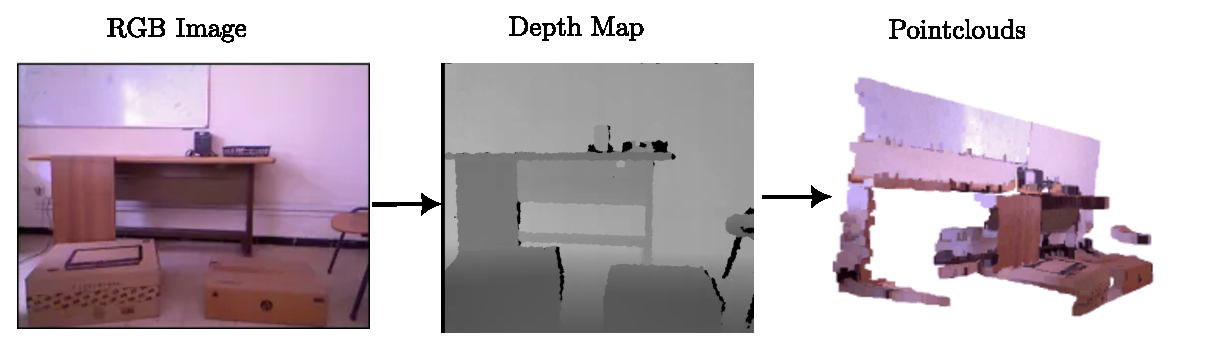
\includegraphics[scale=0.60]{point_cloud.eps}
        \caption{Depth to Pointcloud\footnote{Chayma, et al. Estimate Point Clouds From Depth Images in Python(medium.com)}}
    \end{figure}

    \begin{minipage}{0.47\textwidth}
        \begin{itemize}
            \item The calibration matrix $\mathbf{K}$ is a 3x3 matrix:
        \end{itemize}

        \begin{equation*}
            \mathbf{K} =
            \begin{bmatrix}
                f_x & 0   & c_x \\
                0   & f_y & c_y \\
                0   & 0   & 1
            \end{bmatrix}
            \label{eq:camera_mat}
        \end{equation*}
    \end{minipage}
    \pause
    \begin{minipage}{0.47\textwidth}
        \begin{itemize}
            \item This is the equation for depth to pointcloud
        \end{itemize}
        \begin{equation*}
            \left\{\begin{array}{l}
                z=\operatorname{depth}(i, j)               \\

                x=\dfrac{\left(j-c_x\right) \times z}{f_x} \\
                y=\dfrac{\left(i-c_y\right) \times z}{f_y}
            \end{array}\right.
        \end{equation*}
    \end{minipage}

\end{frame}



\subsection*{Octomap}
\begin{frame}{Octomap}

    % \begin{itemize}
    %     \item An octomap is a data structure and algorithm for efficient 3D mapping for mobile robots.
    %     \item It uses an octree data structure to represent 3D space, dividing it recursively into eight voxels (3D pixels)
    %     \item The leaf nodes of the tree represent small volumes of space, called voxels, which can be used to represent the occupancy of a 3D environment.
    %     \item The tree structure also allows for fast insertion and deletion of objects in the 3D environment, making it well suited for dynamic environments.
    % \end{itemize}

    \begin{itemize}
        \item A mapping framework for efficient 3D mapping.
        \item Octree data structure dividing 3D space recursively into eight voxels.
        \item Leaf node represent small volumes of the space.
        \item Fast insertion and deletion, suitable for dynamic environments.
    \end{itemize}

    \begin{figure}[!ht]
        \centering
        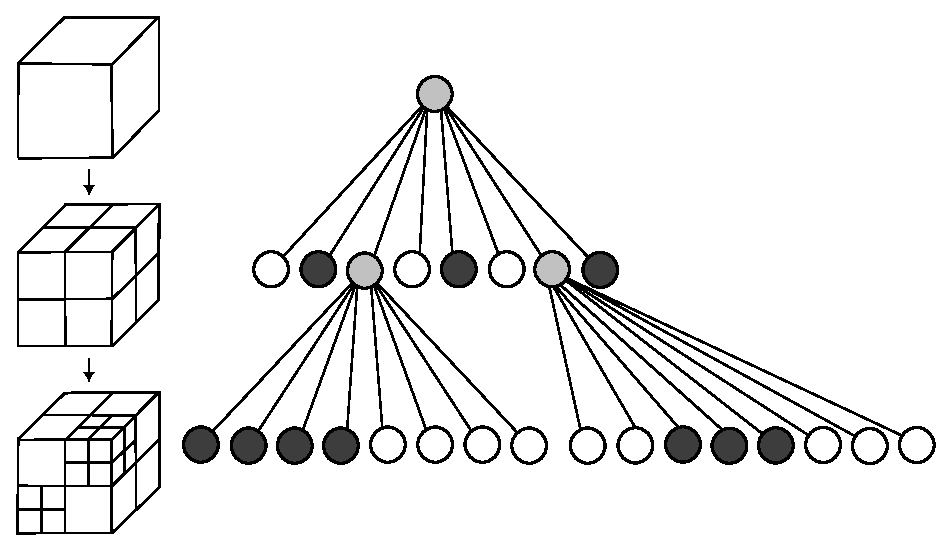
\includegraphics[scale=0.45]{octomap.eps}
        \caption{Octree\footnote{Armin, et al. OctoMap: An Efficient Probabilistic 3D Mapping Framework 2013}}
        \label{fig:octree}
    \end{figure}

\end{frame}
% \subsection*{Probabilistic Sensor Fusion}
% \begin{frame}{Probabilistic Sensor Fusion}

%     \begin{itemize}
%         \item Probabilistic approach to handle uncertainity in the sensor data.
%         \pause
%         \item The probability of a leaf node being occupied, given the sensor measurements up to time t,
%         \begin{equation*}
%             \begin{array}{l}
%                 P\left(n \mid z_{1: t}\right)
%                 \quad=\left[1+\dfrac{1-P\left(n \mid z_t\right)}{P\left(n \mid z_t\right)} \dfrac{1-P\left(n \mid z_{1: t-1}\right)}{P\left(n \mid z_{1: t-1}\right)} \dfrac{P(n)}{1-P(n)}\right]^{-1}
%             \end{array}
%         \end{equation*}
%         \pause
%         \item By using the log-odds notation the equation can be rewritten as 
%         \begin{equation*}
%             \mathrm{L}\left(n \mid z_{1: t}\right)=\mathrm{L}\left(n \mid z_{1: t-1}\right)+\mathrm{L}\left(n \mid z_t\right)
%         \end{equation*}
%         with
%         \begin{equation*}
%             L(n)=\log \left[\frac{P(n)}{1-P(n)}\right]
%         \end{equation*}
%     \end{itemize}
    
% \end{frame}

\subsection*{Motion Planning}
\begin{frame}{Motion Planning}
    \begin{itemize}
        \item Eucledian Signed Distance Fuction(ESDF) based planners.
        \item EGO is ESDF free gradient based planner.
        \item Provides Spline path optimized for smoothness and collisions.
        \item Collision cost as the difference between the collision path and a guiding collision-free path.
        
    \end{itemize}
    \begin{figure}[!ht]
        \centering
        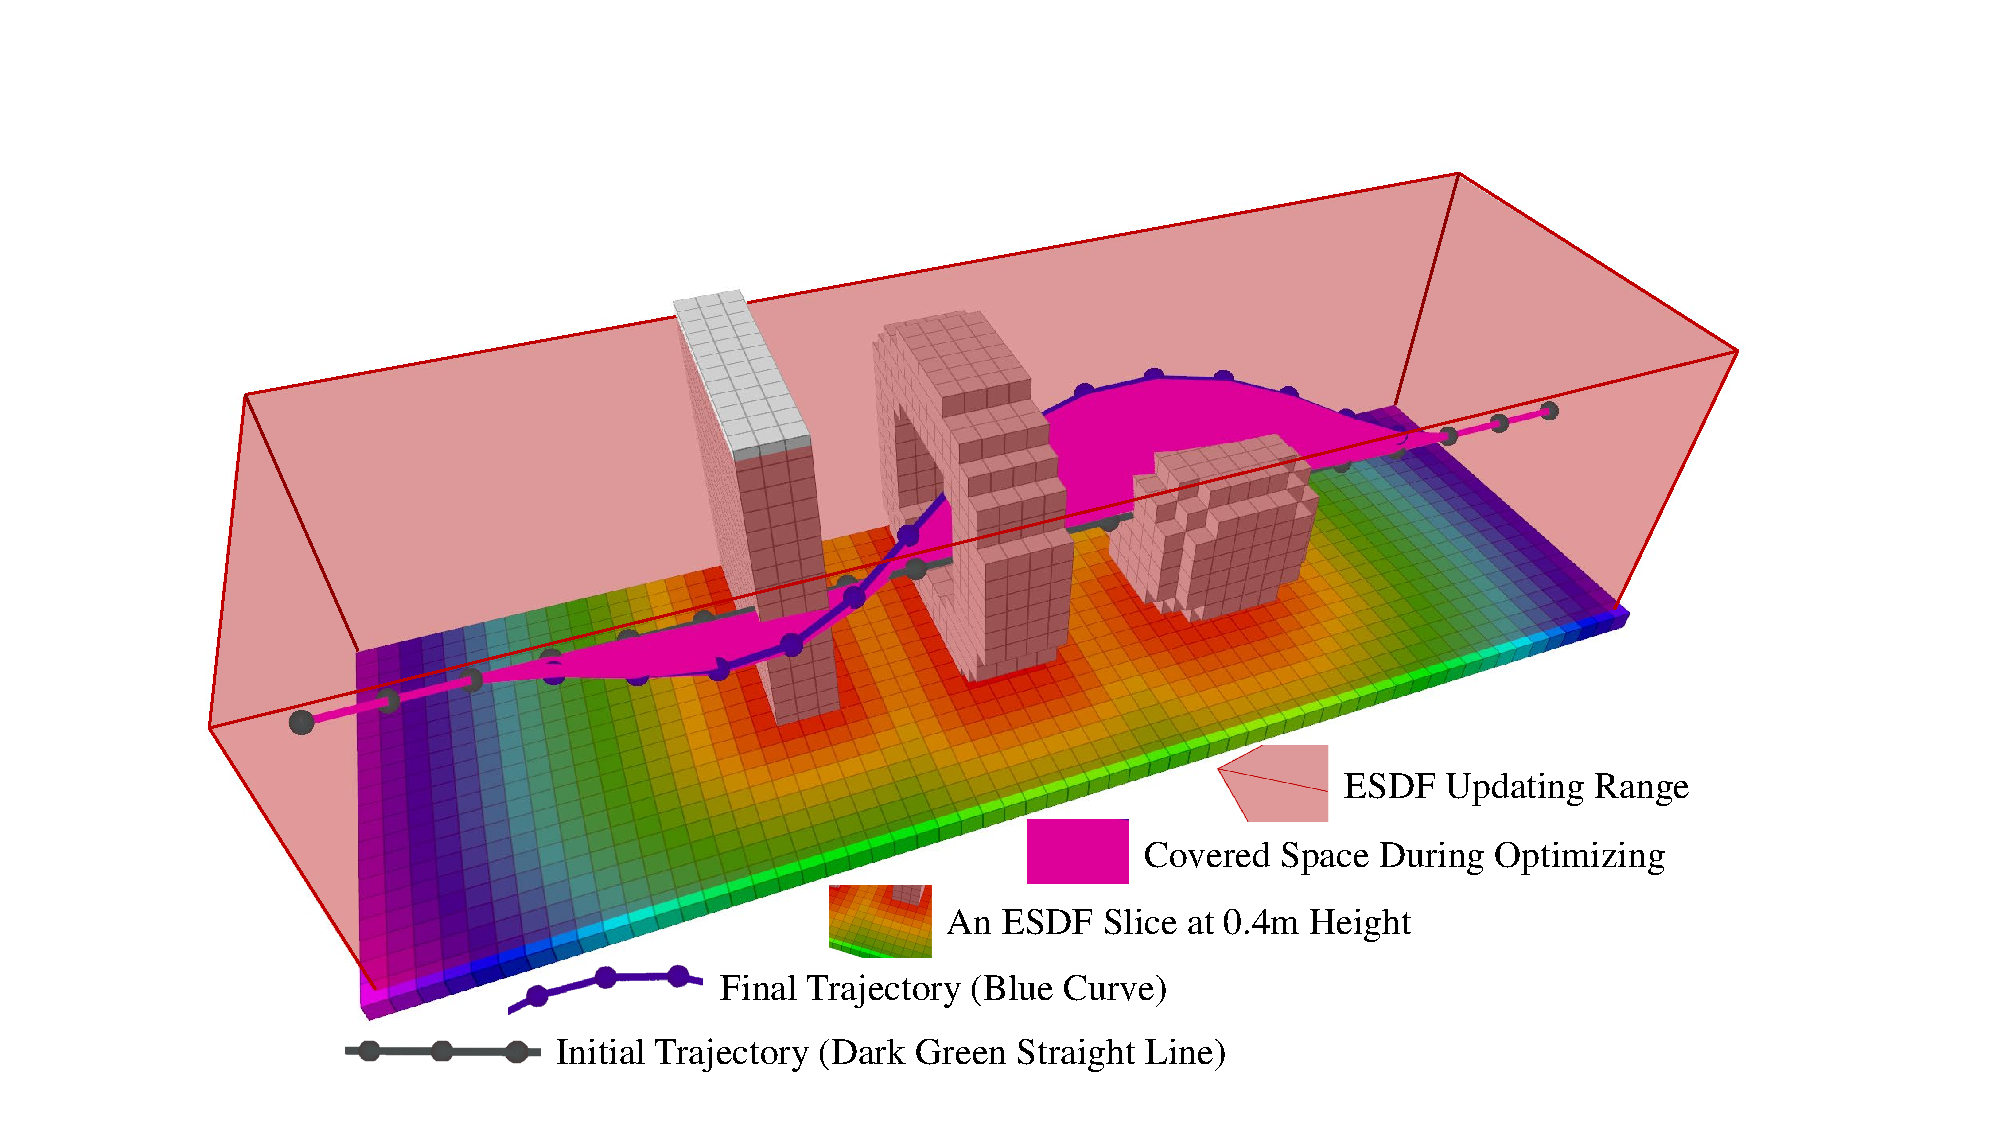
\includegraphics[scale=0.25]{esdf2.pdf}
        \caption{Trajectory by Ego Planner \footnote{X. Zhou, et al. “EGO-planner: An ESDF-free gradient-based local planner for quadrotors,”}}
        \label{fig:ego_planner}
    \end{figure}
\end{frame}

\subsection*{Experiments and Results}

\begin{frame}{Experiments and Results}
    \begin{description}
        \item[Experiment Setup block diagram]
    \end{description}
    \begin{itemize}
        \item The full system block diagram.
    \end{itemize}
    \begin{figure}[!ht]
        \centering
        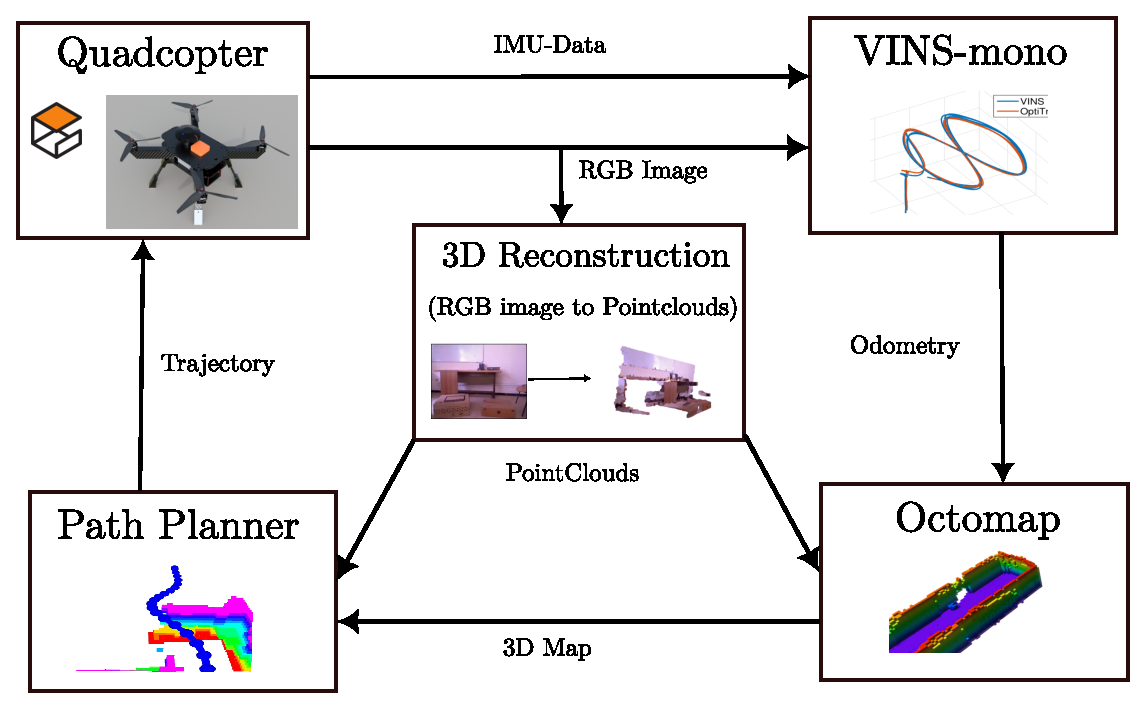
\includegraphics[scale=0.5]{Visual-Pipeline.eps}
        \caption{Full System Pipeline}
        \label{fig:vis_archi_full}
    \end{figure}
\end{frame}


\begin{frame}{}
    \begin{description}
        \item[1. Hardware Configuration]
    \end{description}{}
        \begin{minipage}{0.47\textwidth}
		\begin{enumerate}
    \item \textbf{Raspberry Pi-4 : }
    \begin{itemize}
        \item 4 GB of DDR4 RAM and 1.5 GHz clock
        \item Quad core Cortex-A72 (ARM v8) 64-bit SoC
    \end{itemize}

    \item \textbf{Pixhawk 2.4.8 FCU : }
    \begin{itemize}
        \item 32bit STM32F427 Cortex M4 core with FPU with 168 MHz clocks
        \item ST Micro L3GD20H 16-bit gyroscope
        \item ST Micro X4HBA 303H 14-bit accelerometer
    \end{itemize}

    \item \textbf{ : Raspberry Pi Cam V-2 }
    \begin{itemize}
        \item Sony IMX219 8-MP sensor
        \item 1080 at 30 Hz, 720 at 60 Hz
    \end{itemize}  
\end{enumerate}
	\end{minipage}
	\begin{minipage}{0.47\textwidth}
		\begin{figure}[h!]
			\centering
			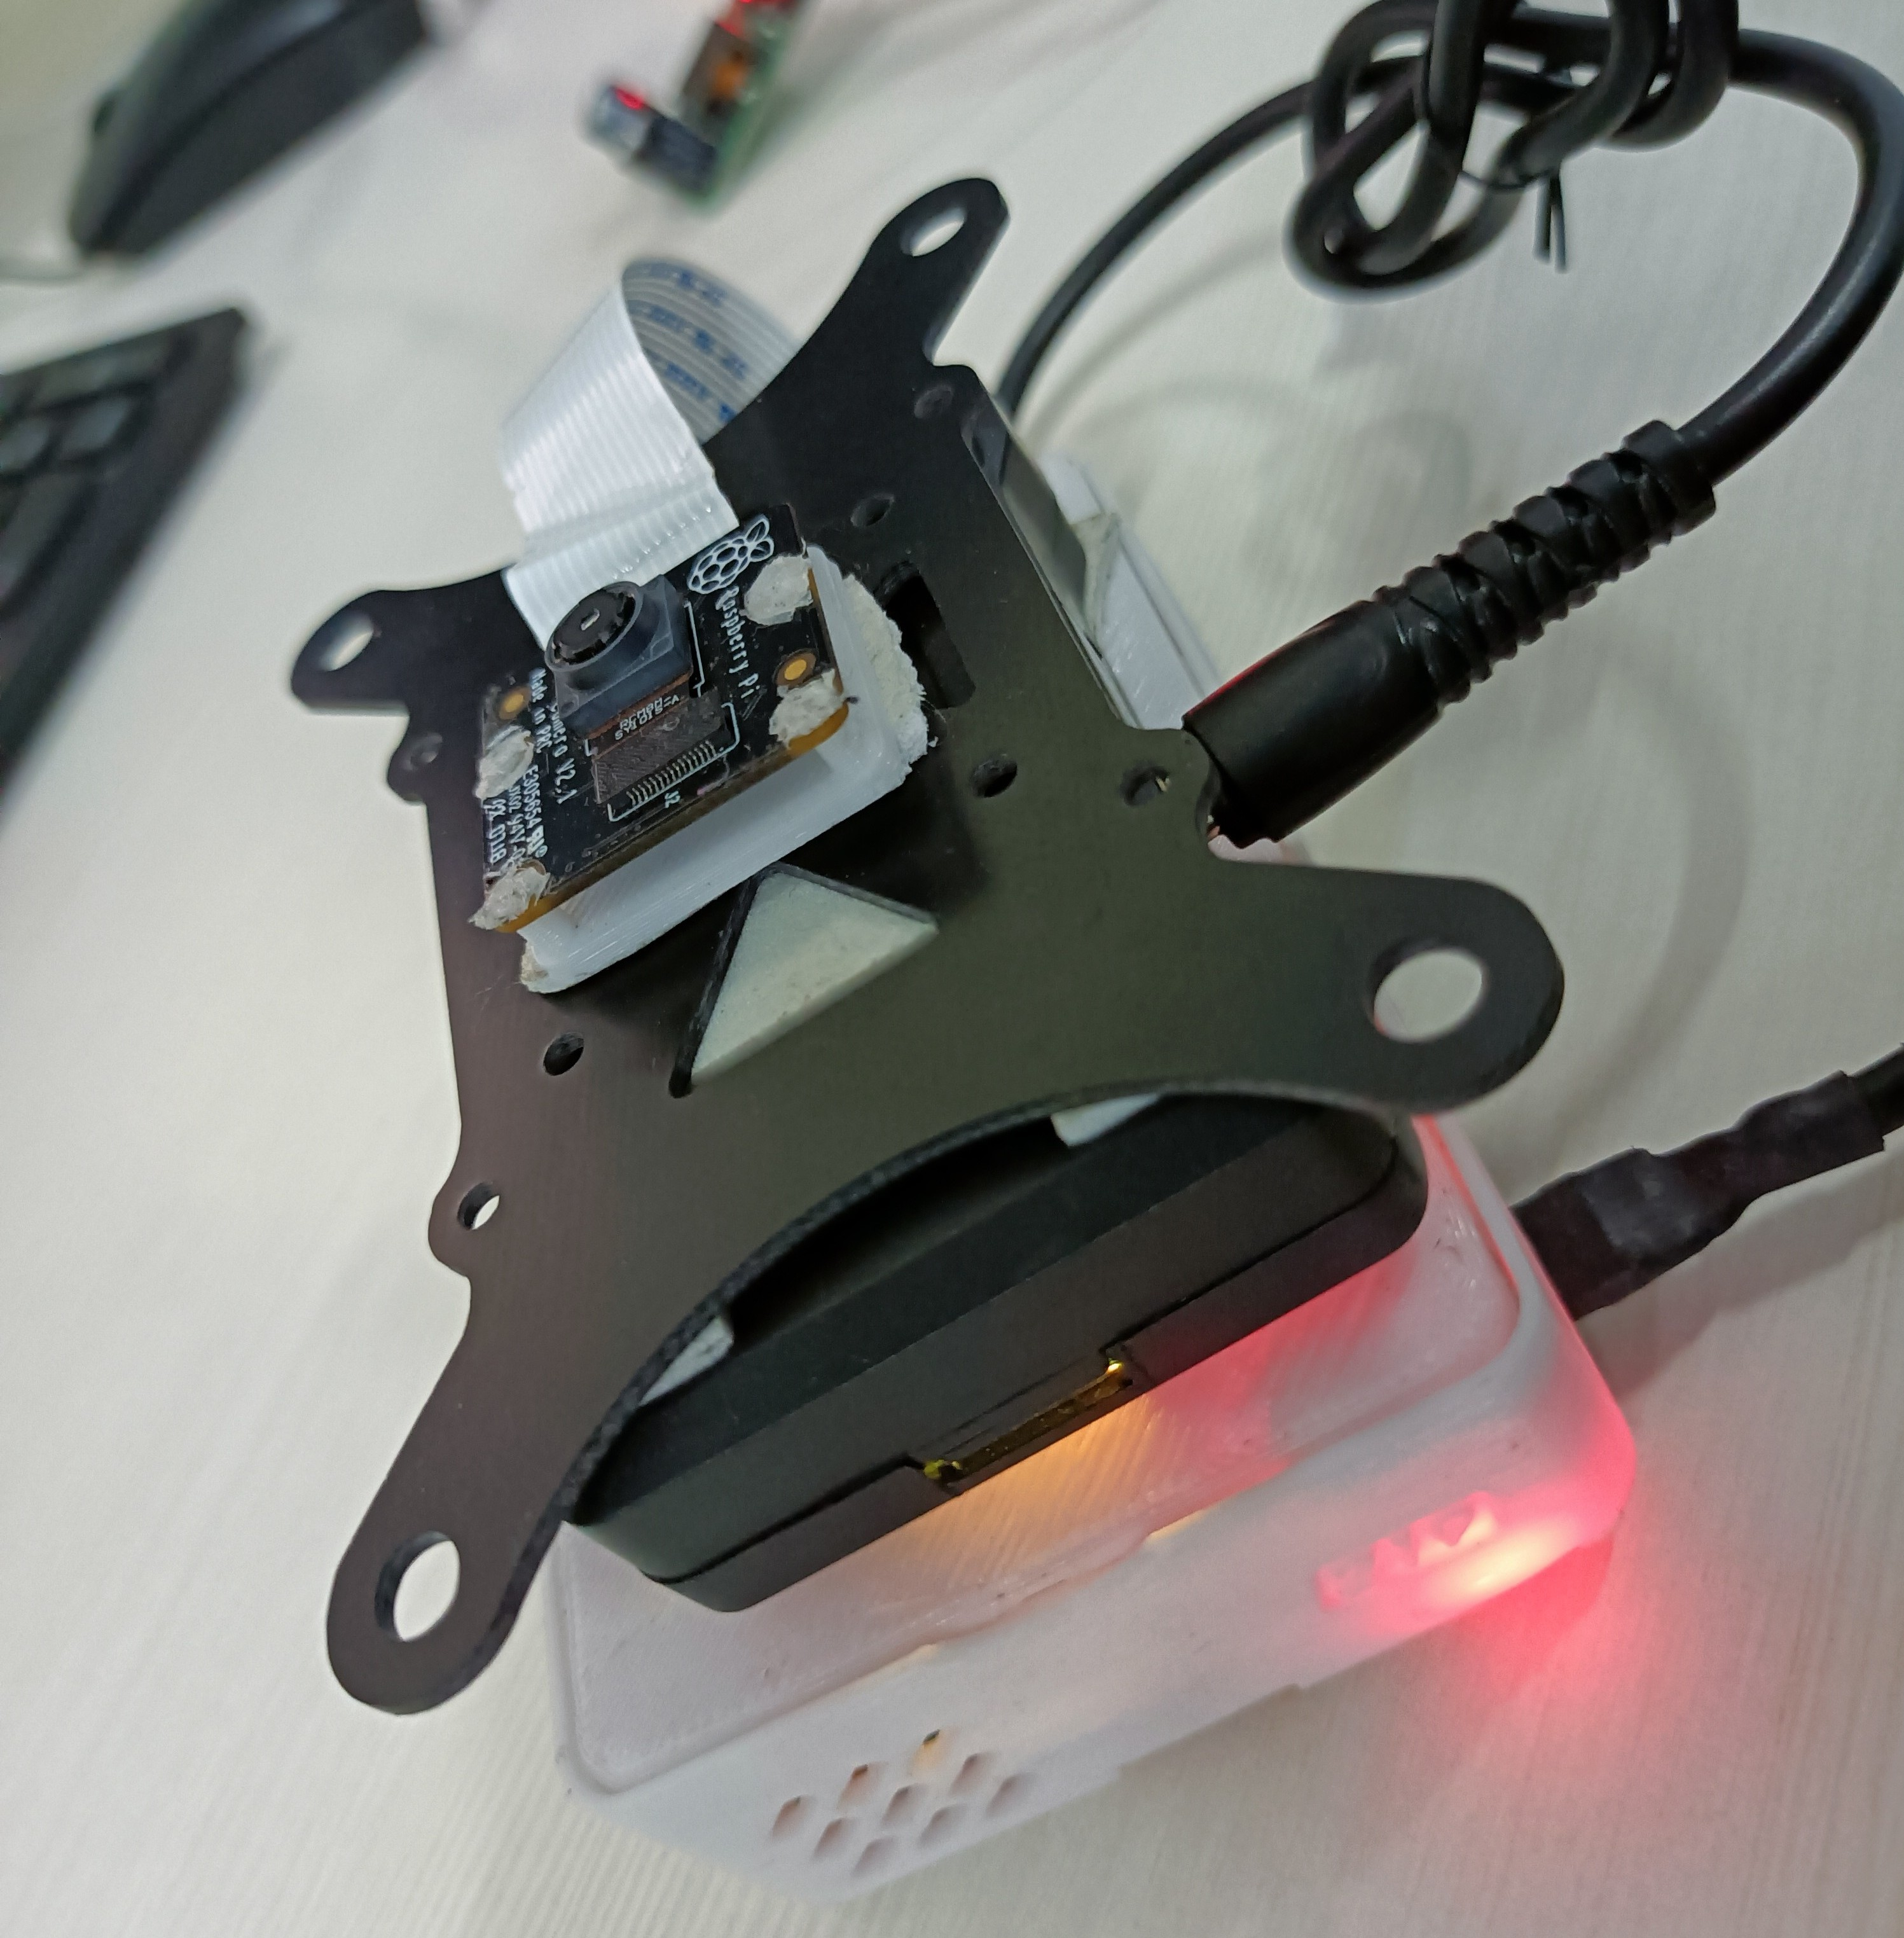
\includegraphics[scale=0.05]{VIO_module_1.jpg} 
			\caption{Hardware Module for VIO}
			\label{Fig:VIO_hardware_module}
		\end{figure}
	\end{minipage}
\end{frame}
\begin{frame}{}
    \begin{description}
        \item[2. Camera Calibration]
    \end{description}{}
        \begin{minipage}{0.47\textwidth}
\begin{itemize}
    \item Intrinsic Camera Matrix \\
    
    $$\mathbf{K} = \begin{bmatrix}
        501 & 0 & 318\\
        0  & 500 & 223 \\
        0 & 0 & 1
    \end{bmatrix}$$
    \item Distortion parameters 
    $$\begin{bmatrix}
        \mathbf{k1}\\
        \mathbf{k2}\\
        \mathbf{p1}\\
        \mathbf{p2}\\
        \mathbf{p3}
    \end{bmatrix} =  \begin{bmatrix}
        0.1569\\
        -0.272\\
        -1.5e-4\\
        -7.33e-04\\
        0
    \end{bmatrix}$$

\end{itemize}
	\end{minipage}
	\begin{minipage}{0.47\textwidth}
		\begin{figure}[h!]
			\centering
			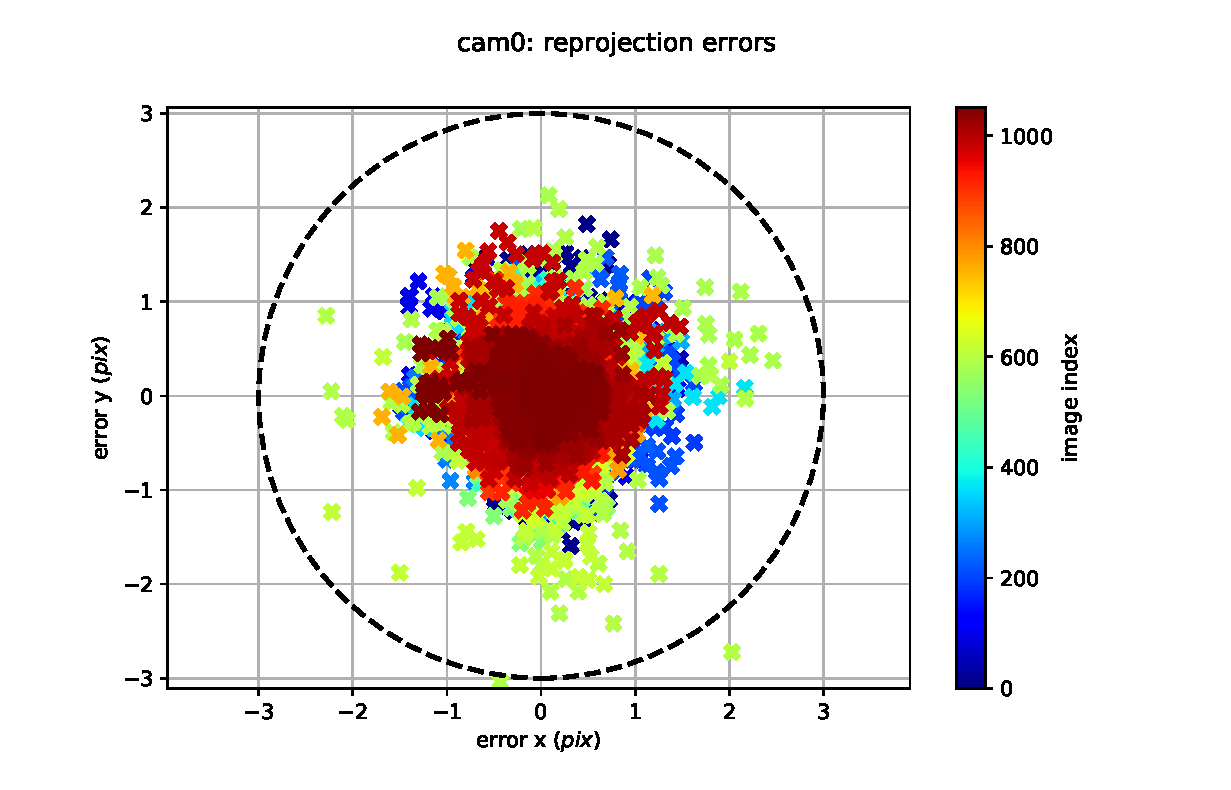
\includegraphics[scale=0.35]{Camera_Reprojection.eps} 
			\caption{Camera Reprojection error}
			\label{Fig:cam_reproj}
		\end{figure}
	\end{minipage}
        \begin{itemize}
    \item Transformation matrix $\mathbf{T}_{b}^{c} = \begin{bmatrix}
        0.013 & 0.999 & 0.0532  & -0.044\\
       0.998 & -0.014 & 0.007  & 0.007\\ 
       0.008 & 0.053 &  -0.998 & -0.082\\
       0 & 0 & 0 & 1
    \end{bmatrix}$
\end{itemize}
\end{frame}

\begin{frame}{}
\begin{description}
    \item[3. VIO Experiment]
\end{description}
        \begin{itemize}
            \item The experiment is conducted in SP14 lab
            \item VIO experiment with 56.82 meters long trajectory is evaluated   
            \item The RMSE error is 0.38 and 0.57 along the x and y axis respectively
            \item The total drift is 1.2 meters along the y-axis
        \end{itemize}{}
            \begin{figure}[h!]
			\centering
			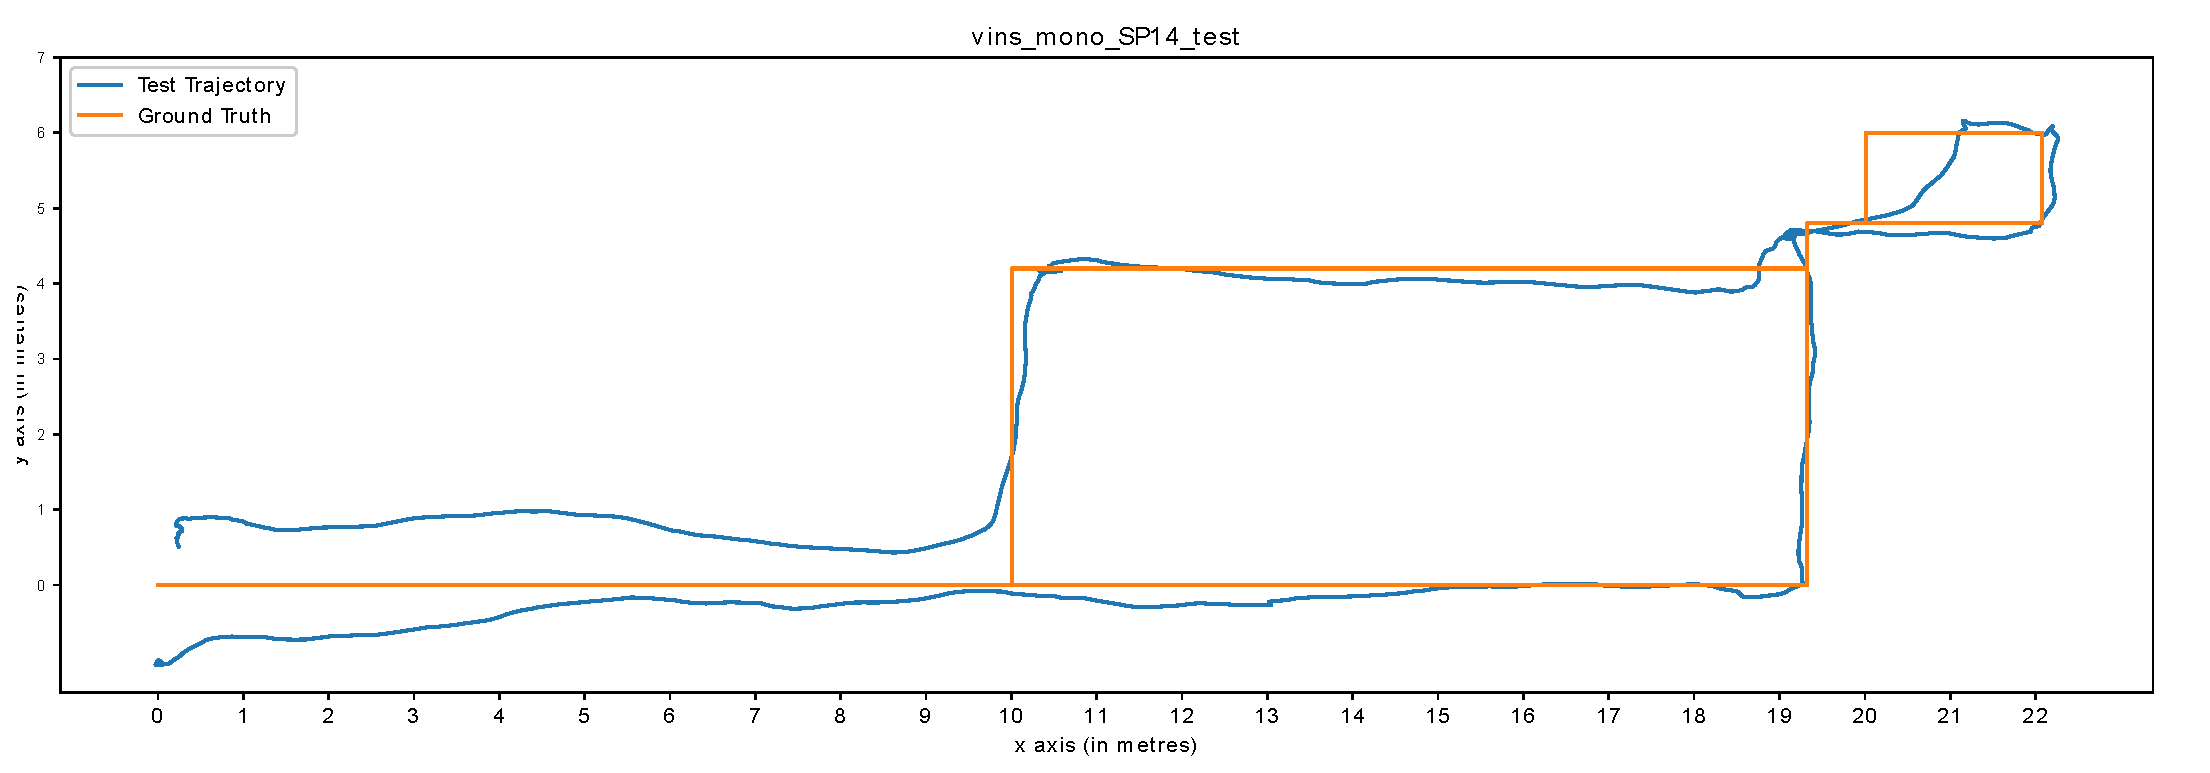
\includegraphics[scale=0.32]{vins_mono_SP14_test.eps} 
			\caption{VINS-mono SP14}
			\label{Fig:vins_mono}
		\end{figure}
\end{frame}

\begin{frame}{}
    \begin{description}
        \item[4. Mapping]
    \end{description}
    \begin{itemize}
        \item Odomery from VINS-mono and pointcloud from 3D dense reconstruction is used.
        \item The experiment is conducted in SP14 lab
        \begin{figure}[!ht]
            \centering
            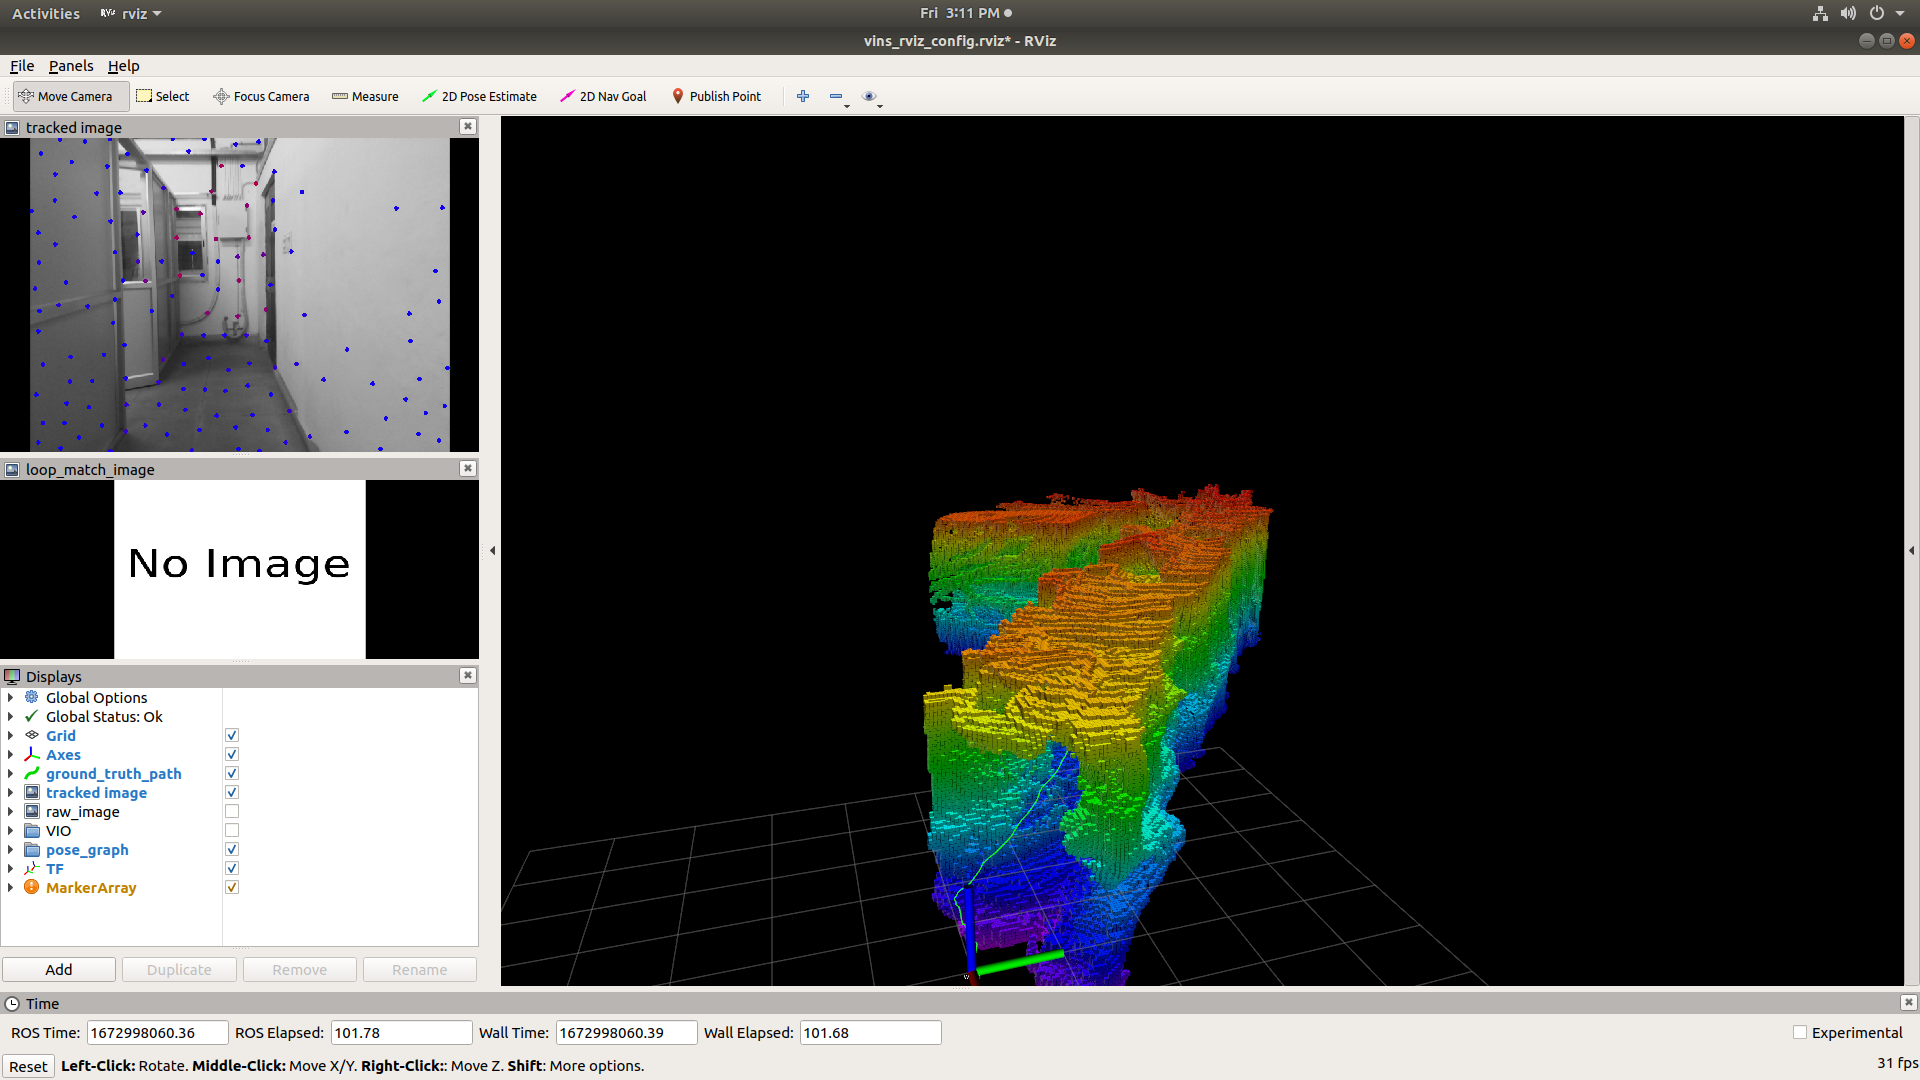
\includegraphics[scale=0.11]{Octomap_Sp14-2.png}
            \caption{Octomap in Sp14 using monocular RGB camera}
            \label{fig:octomap_sp14}
        \end{figure}
    \end{itemize}
\end{frame}

\begin{frame}{}
    \begin{description}
        \item[5. Motion Planning]
    \end{description}
    \begin{itemize}
        \item Simulated in ROS Gazebo.
        \item System pipeline is implemented using XTDrone package.
        \item XTDrone provides modular drone framework.
        \item Used PX4 SITL for quadcopter
        \item The full video is \includemovie[
            poster,
            autoplay,
            externalviewer,
            inline=true,
            text={ i}
            ]{0.3cm}{0.3cm}{xt_drone.mp4} 
    \end{itemize}
    \begin{figure}[!ht]
        \centering
        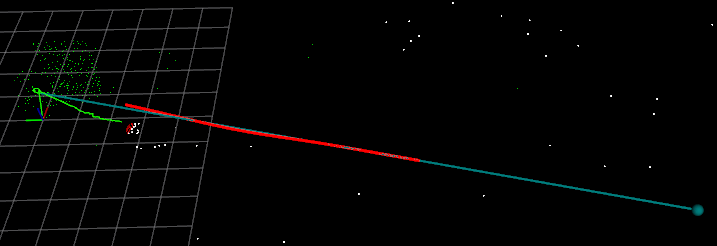
\includegraphics[scale=0.4]{startraj-1.png}
        \caption{Autonomous Navigation in Simulation}
        \label{fig:xtdrone}
    \end{figure}
    
\end{frame}

\begin{frame}{}
    \begin{description}
        \item[6. Computational Analysis]
    \end{description}
    \begin{minipage}{0.47\textwidth}

        \begin{figure}[h!]
            \centering
            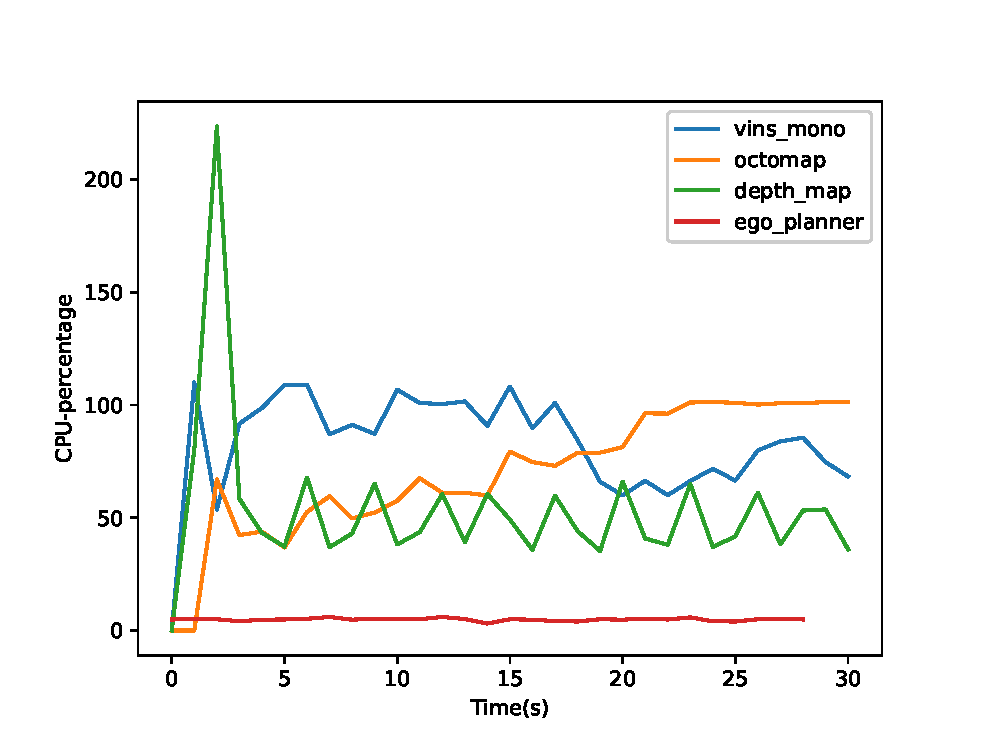
\includegraphics[scale=0.40]{computation.eps}
            \caption{CPU Usage Analysis}
        \end{figure}
    \end{minipage}
    \begin{minipage}{0.47\textwidth}

        \begin{figure}[h!]
            \centering
            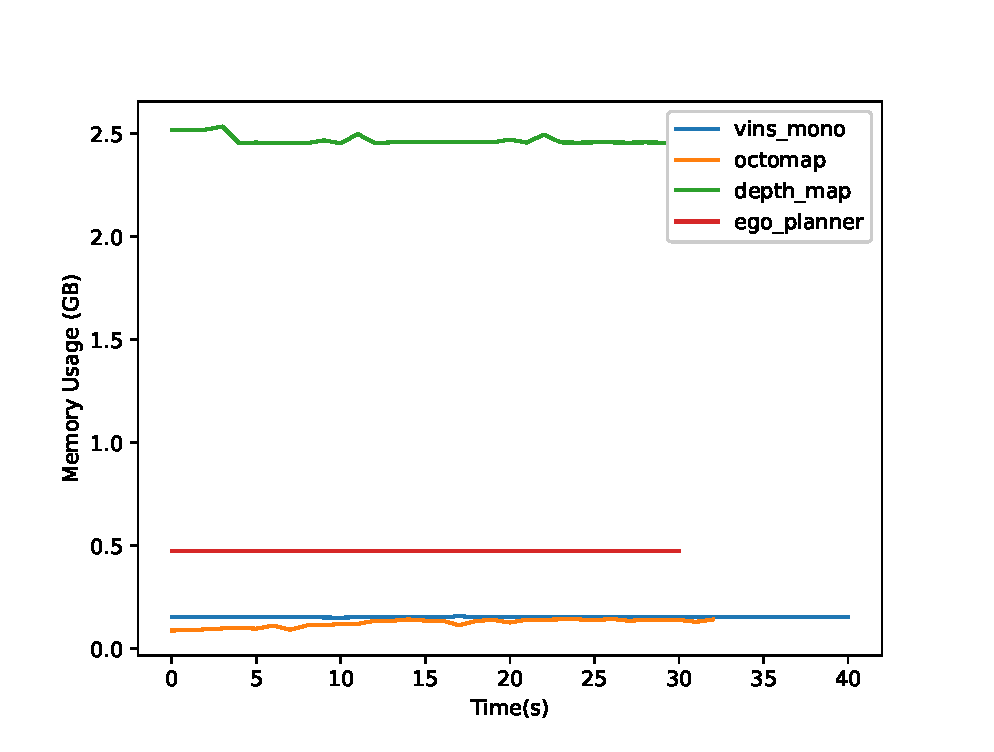
\includegraphics[scale=0.40]{memory.eps}
            \caption{Memory Usage}
        \end{figure}
    \end{minipage}

This work is submitted as:

\hspace{0.8cm}Arvind Pandit, Om Patil, Ameer K. Mulla, ``\textbf{MoVINav}-A \textbf{Mo}nocular \textbf{V}isual \textbf{I}nertial \textbf{Nav}igation Framework", in \textit{62nd IEEE Conference on Decision and Control}, Singapore.(Under Review)

\end{frame}
\section*{}
\begin{frame}{}
    \huge{\centerline{\textcolor{blue}{\textbf{3. Monocular Thermal Navigation }}}}
\end{frame}

\section{Monocular Thermal Inertial Navigation System}
\subsection*{Sensor Evaluation}
\begin{frame}{Sensor Evaluation}
    \begin{itemize}
        \item Radar and LWIR camera are suitable in a smoke environment \footnote{J W. Starr,et al. Evaluation of Navigation Sensors in Fire Smoke Environments, 2013.}
    \end{itemize}
    \begin{figure}[h!]
        \centering
        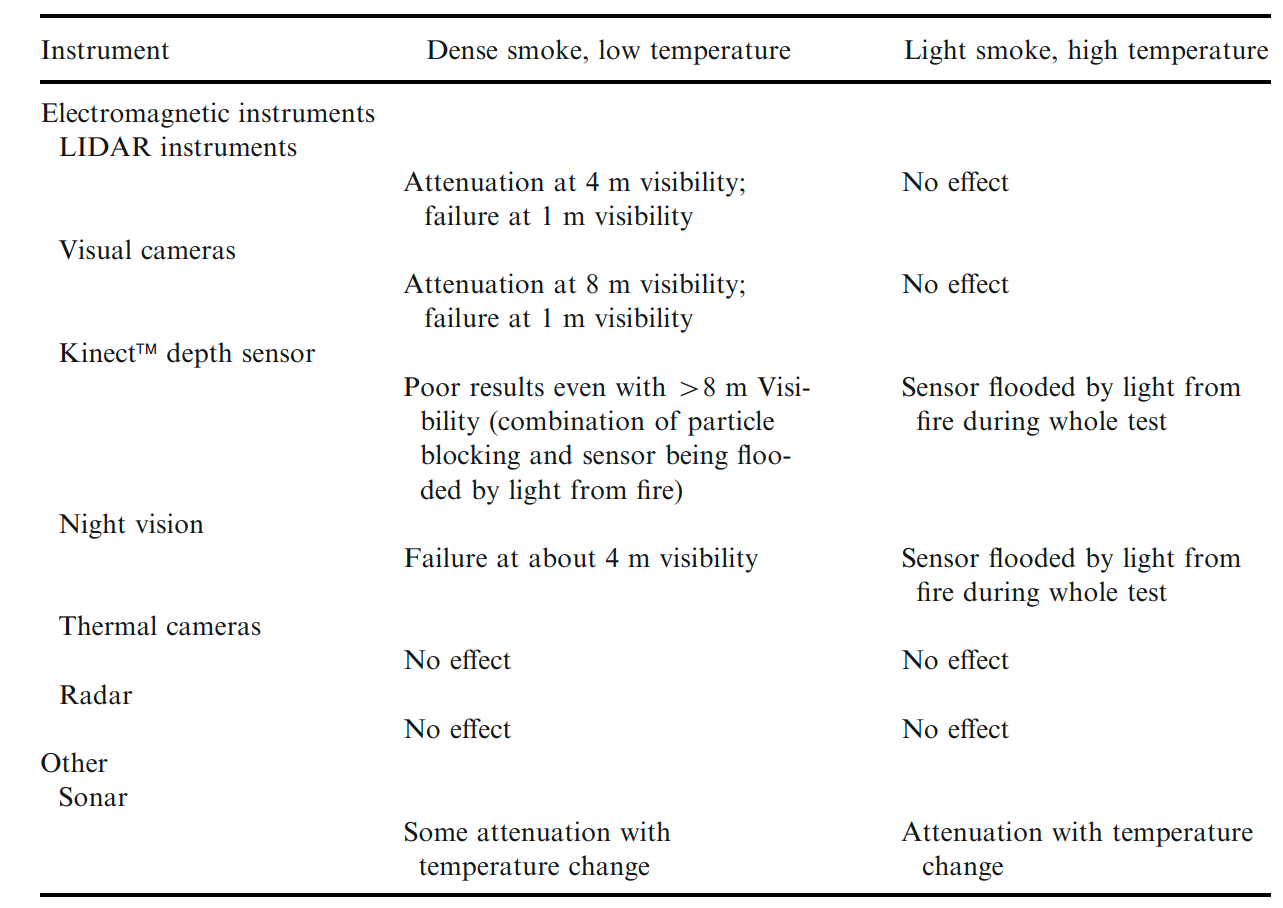
\includegraphics[scale=0.20]{Navigaion_sensor.png}
        \label{Fig:nav_eval}
    \end{figure}
\end{frame}

\subsection*{Camera Module}
\begin{frame}{Camera Module}

    \begin{itemize}
        \item FLIR Tau 2 640x512 LWIR camera , 30Hz frequency. 
        \item The Cube Orange flight controller, 32bit ARM STM32H753 Cortex-M7 and 400MHz clock.
        \item A custom PCB is designed to reduce the hardware of the system.
    \end{itemize}

    \begin{figure}[!ht]
        \centering
        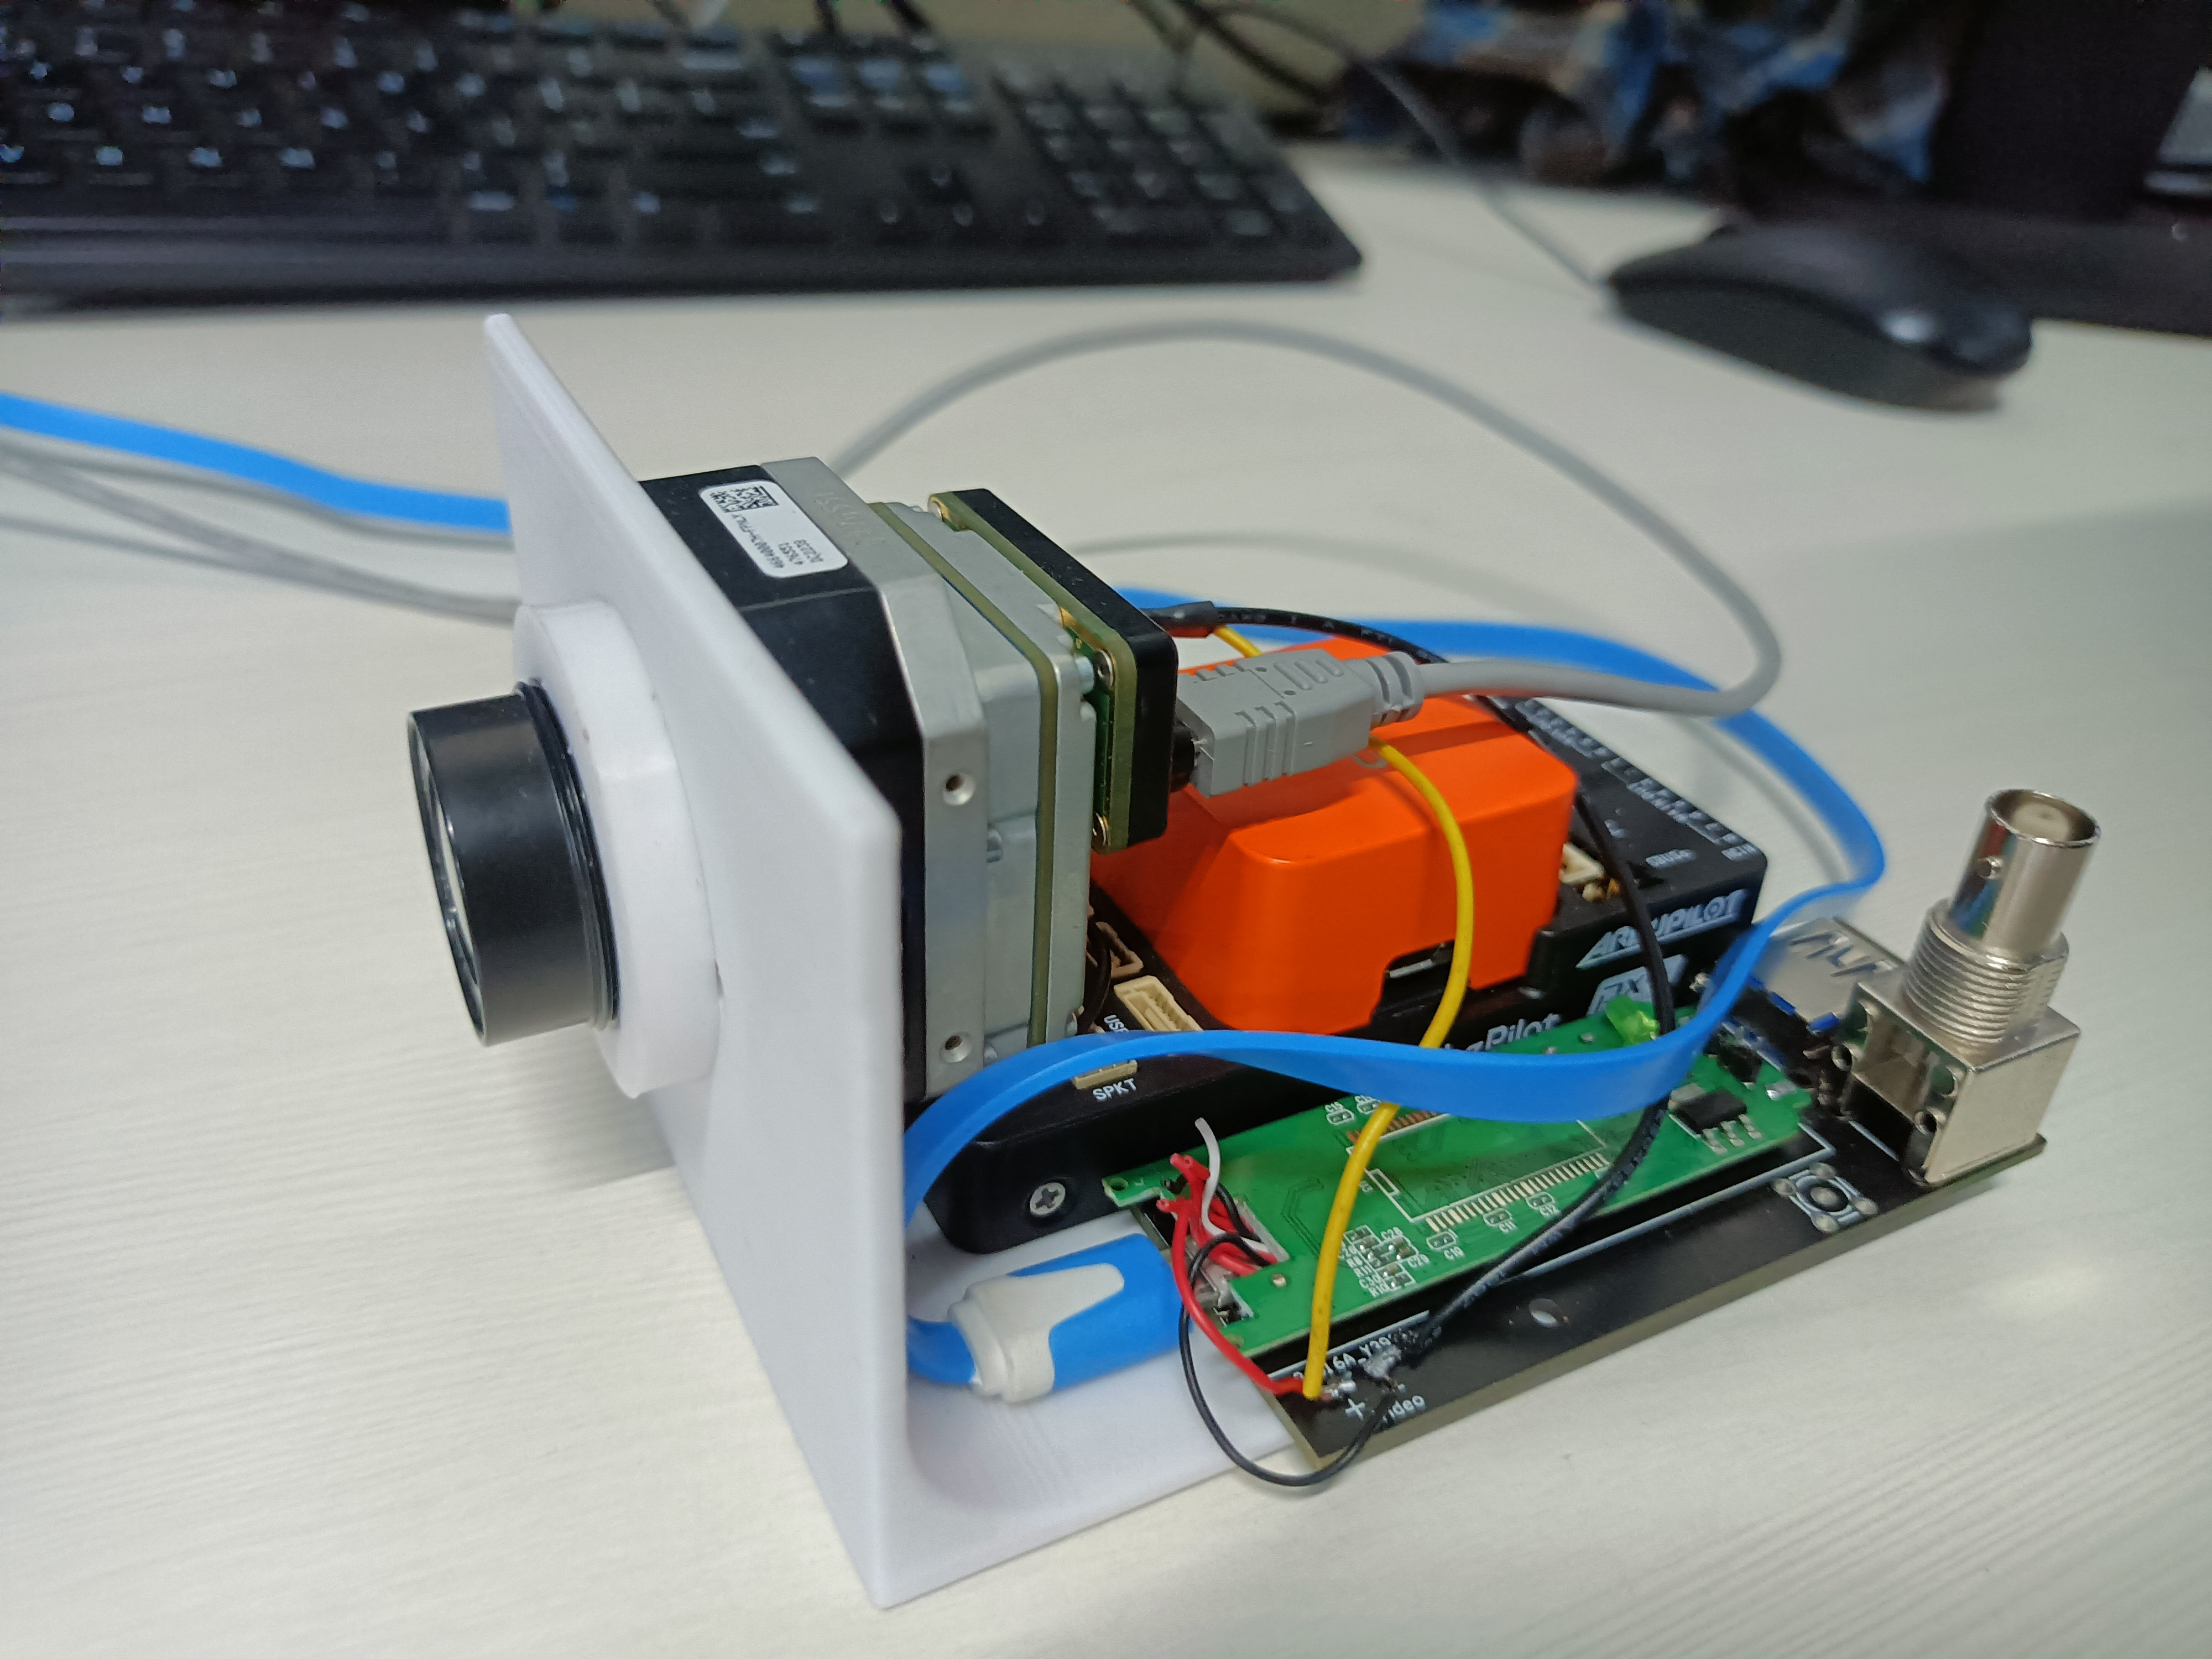
\includegraphics[scale=0.045]{TIO_module.jpg}
        \caption{Thermal Inertial Odometry Module}
        \label{fig:TIO_module}
    \end{figure}
\end{frame}

\subsection*{Thermal Camera Calibration}
\begin{frame}{Thermal Camera Calibration}
    \begin{minipage}{0.47\textwidth}

        \begin{figure}[h!]
            \centering
            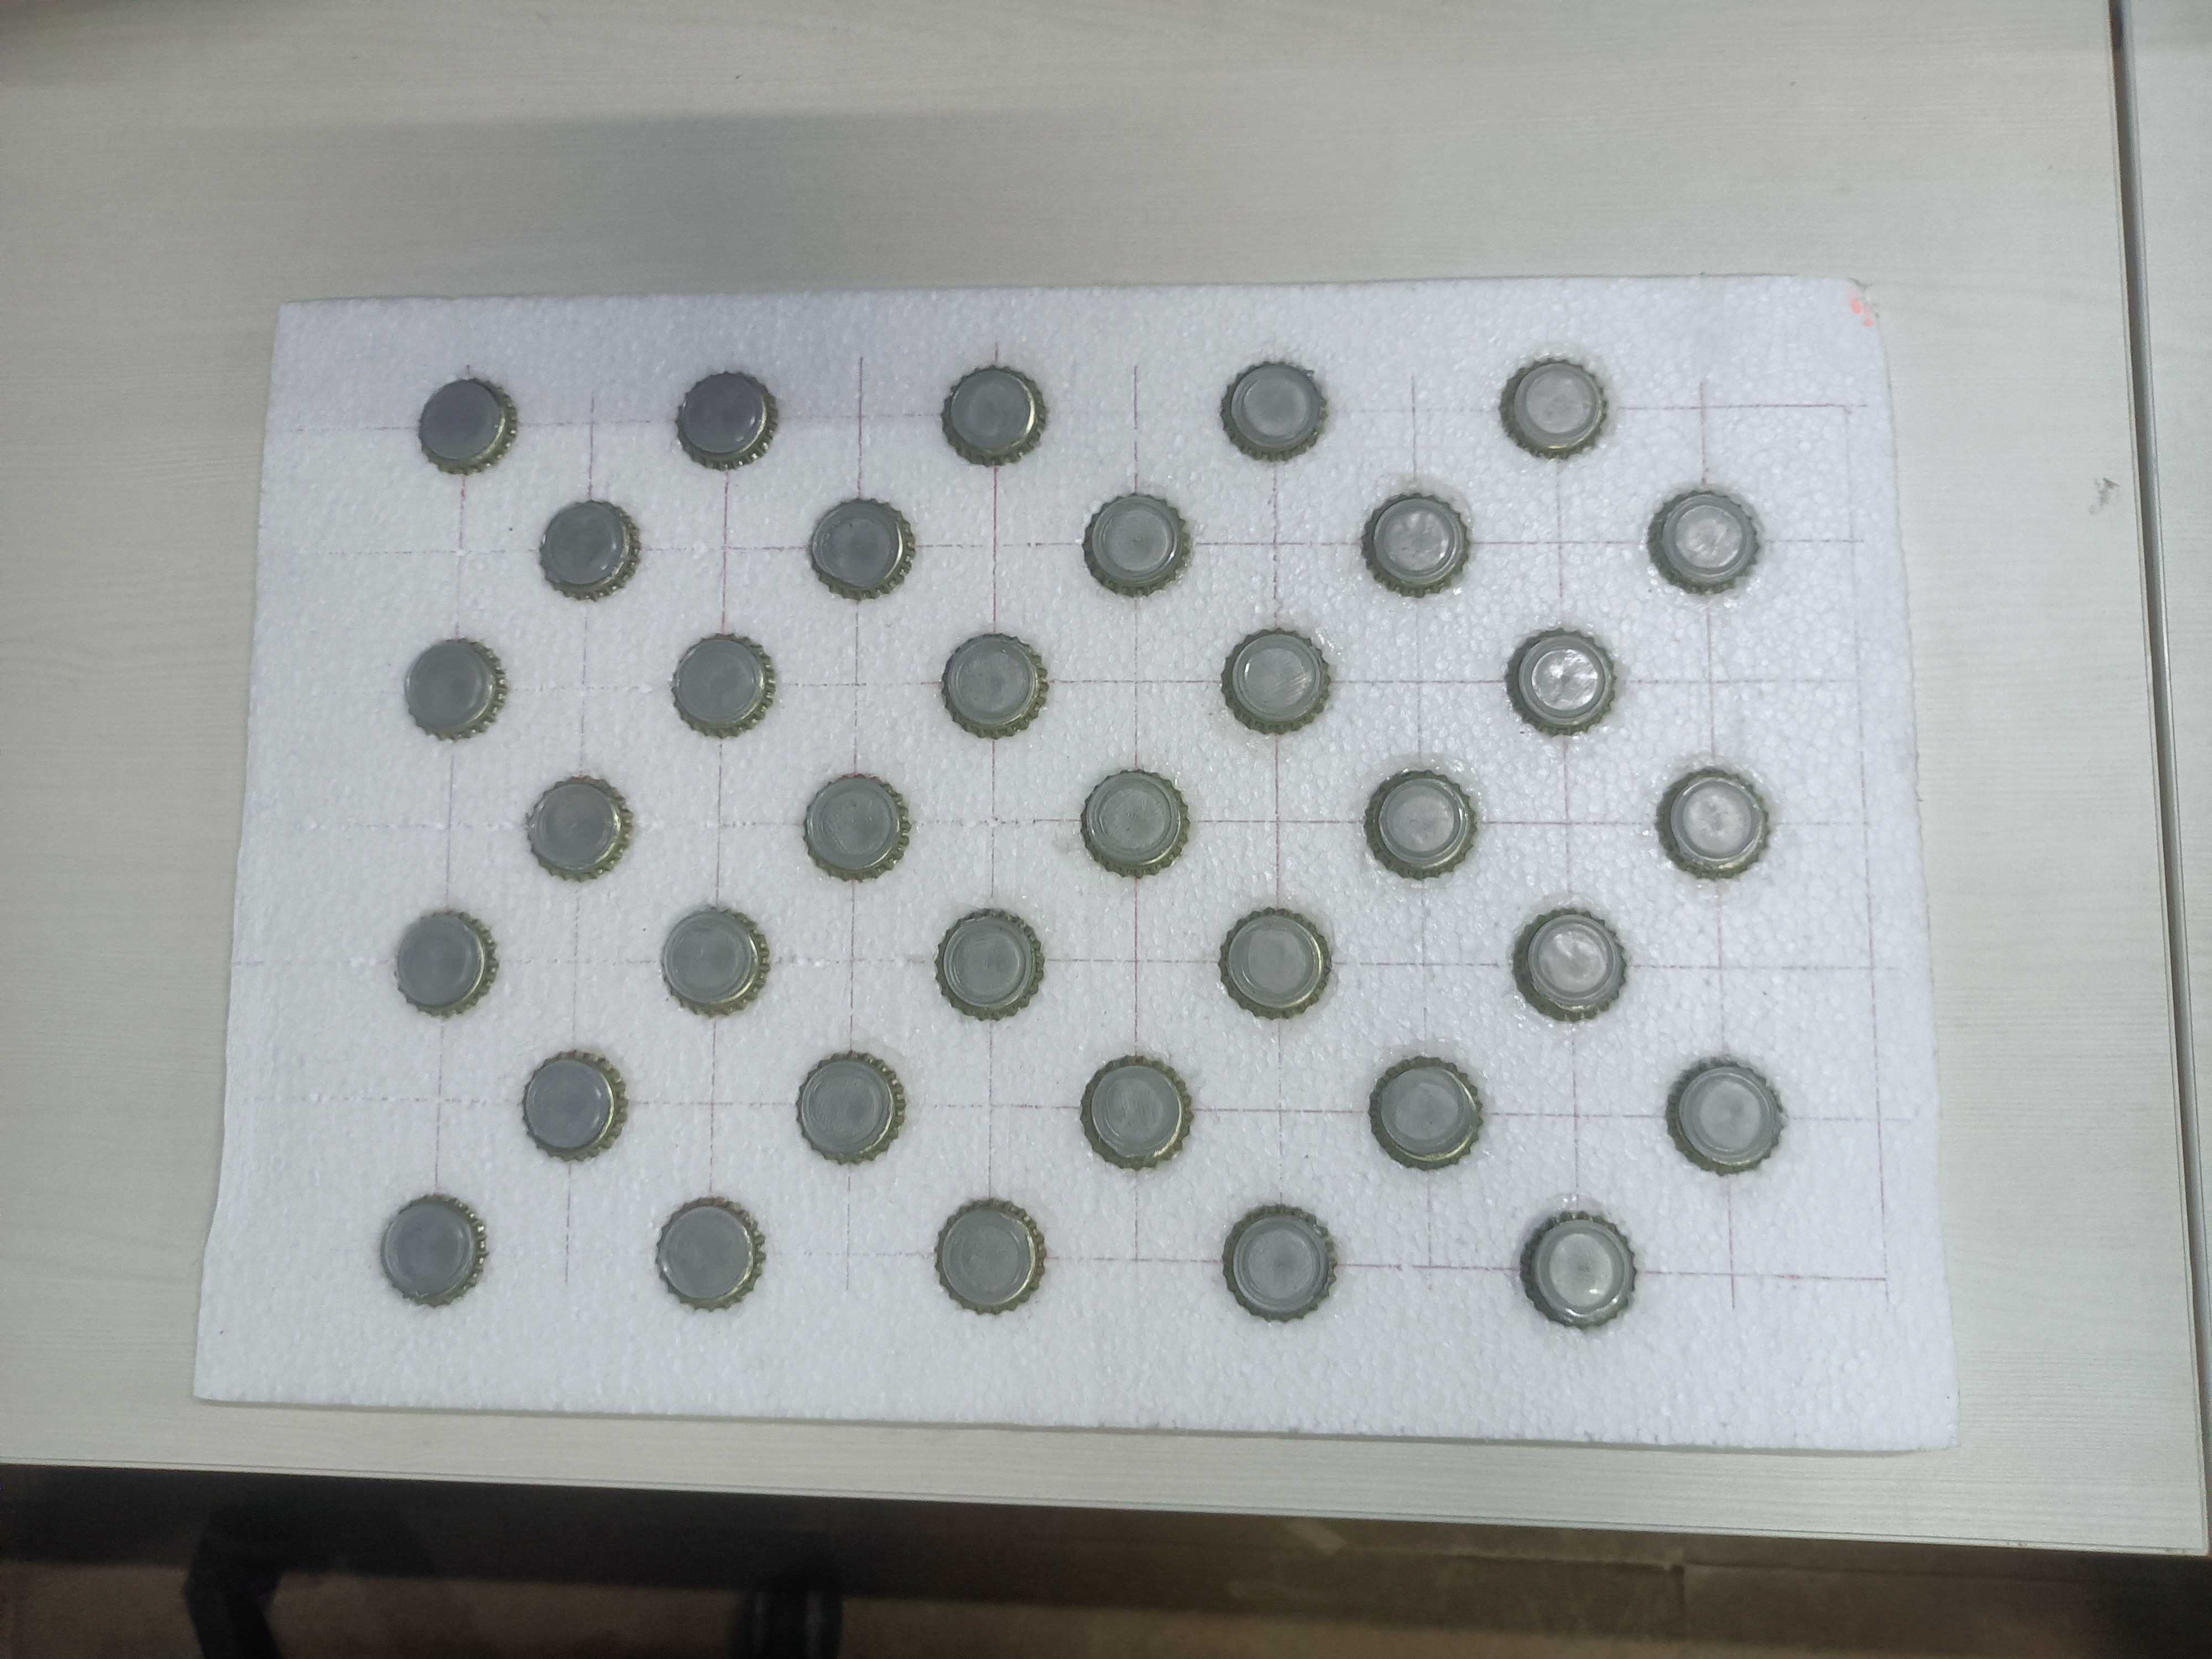
\includegraphics[scale=0.03]{Calibration_board.jpg}
            \caption{Calibration Board}
            \label{fig: calib_board}
        \end{figure}

    \end{minipage}
    \begin{minipage}{0.47\textwidth}
        \vspace{0.2cm}
        \begin{figure}[h!]
            \centering
            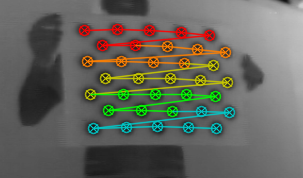
\includegraphics[scale=0.5]{Corner_detected_thermal.png}
            \caption{Grid detection in LWIR camera}
            \label{fig: grid_detection}
        \end{figure}

    \end{minipage}
    \begin{itemize}
        \item Custom asymmetric circle grid calibration board is fabricated.
        \pause
        \item Two materials with different emmisivity and thermal radiation property.
        \item The circles are made of iron having low emmisivity  on background of foam sheet with higher value.
        \pause
        \item The Kalibr calibration framework is used for the calibration of an intrinsic parameters of the LWIR camera.\footnote{Joern, et al. Extending kalibr, 2016}
    \end{itemize}
\end{frame}

\subsection*{Thermal Odometry}
\begin{frame}{Thermal Odometry}
    \begin{itemize}
        \item Capture images: $I_t$ and $I_{t + 1}$
        \item Undistort the captured images.
        \item Use SURF detector algorithm to detect features in image $I_t$. 
        \item Track these features using an optical flow methodology, remove points that fall out of frame or are not visible in $I_{t + 1}$. 
        \item Trigger a new detection of points if the number of tracked points falls behind a threshold. Set to 100 in this implementation.
        \item Nister's 5-point algorithm with RANSAC to find the essential matrix.
        \item Estimate R, t from the essential matrix.
        \begin{figure}[h!]
            \centering
            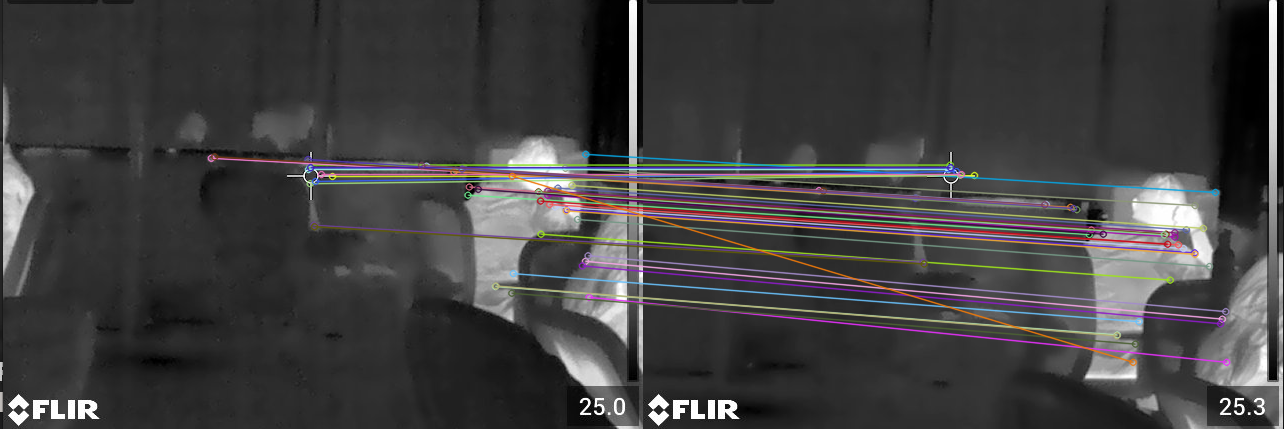
\includegraphics[scale=0.20]{Thermal_feature_matching.png}
            \caption{Feature detection and matching}
            \label{fig: tio}
        \end{figure}
    \end{itemize}
\end{frame}

\subsection*{Thermal Human Detection}
\begin{frame}{Thermal Human Detection}
    \begin{minipage}{0.47\textwidth}
        \begin{figure}[h!]
               \centering
               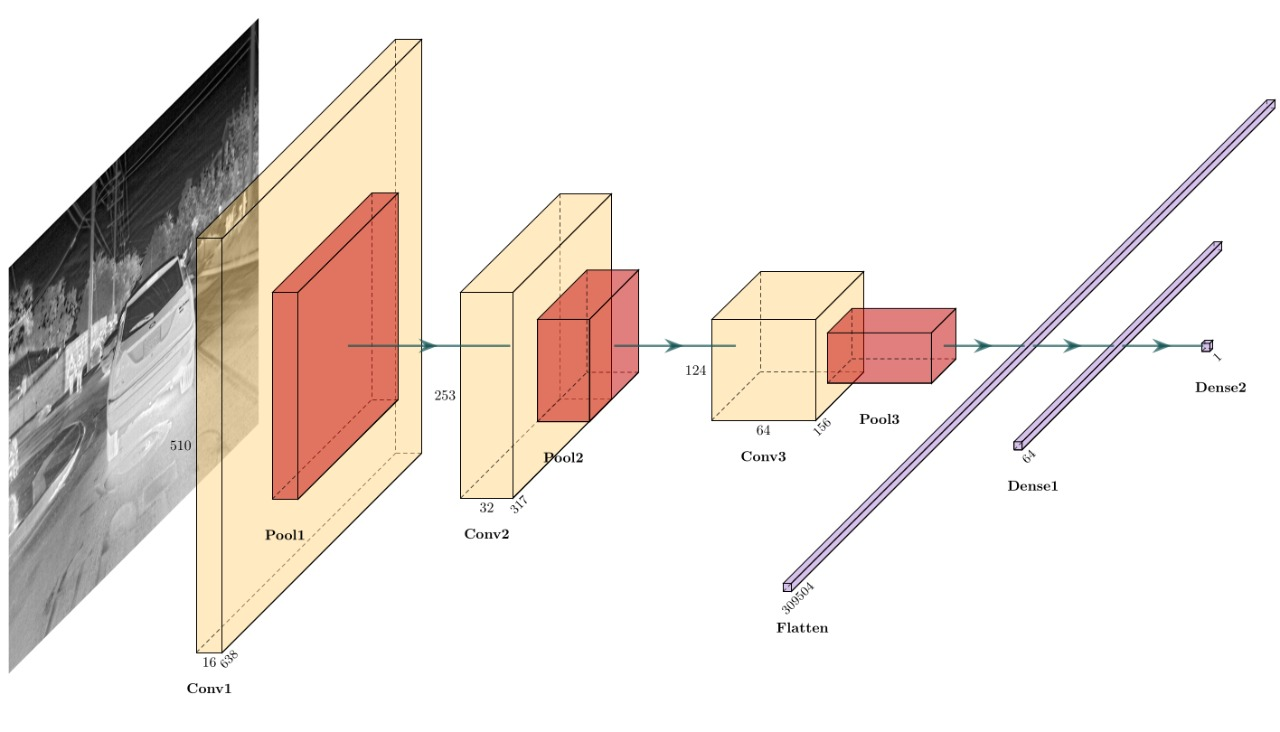
\includegraphics[scale=0.095]{NN.jpeg}
               \caption{CNN model}
               \label{Fig:NN}
           \end{figure}
       \end{minipage}
       \begin{minipage}{0.47\textwidth}
                \begin{figure}[h!]
               \centering
               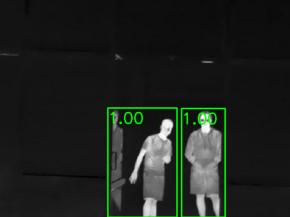
\includegraphics[scale=0.3]{272.png} 
               \caption{Human detection }
               \label{Fig:human_detec}
           \end{figure}
       \end{minipage}

    \vspace{-0.2cm}
    \begin{table}[!ht]
		\centering
		\resizebox{0.47\textwidth}{!}{\begin{tabular}{|l|l|l|l|}
			\hline
			Model    & Accuracy        & AUROC           & BCE             \\ \hline
			ResNet18 & 0.9767          & 0.9980          & 0.0541          \\ \hline
			ResNet34 & \textbf{0.9917} & \textbf{0.9992} & \textbf{0.0295} \\ \hline
			ResNet50 & 0.9827          & 0.9989          & 0.0504          \\ \hline
		\end{tabular}}
		\label{tab:classification_performance}
	\end{table}
    \pause
	\begin{table}[!ht]
		\centering
		\resizebox{0.80\textwidth}{!}{\begin{tabular}{|l|lll|}
			\hline
			\multirow{2}{*}{Device}       & \multicolumn{3}{c|}{Throughput (FPS)}                                    \\ \cline{2-4} 
										  & \multicolumn{1}{l|}{ResNet18} & \multicolumn{1}{l|}{ResNet34} & ResNet50 \\ \hline
			Raspberry Pi 4 (4 GB)            & \multicolumn{1}{l|}{9.20}    & \multicolumn{1}{l|}{6.42}    & 4.31    \\ \hline
			Jetson Nano (4 GB)            & \multicolumn{1}{l|}{47.70}    & \multicolumn{1}{l|}{26.96}    & 14.41    \\ \hline
			Jetson Nano TensorRT (4 GB)   & \multicolumn{1}{l|}{88.10}    & \multicolumn{1}{l|}{50.10}    & 32.53    \\ \hline
			Nvidia RTX3060                & \multicolumn{1}{l|}{755.52}   & \multicolumn{1}{l|}{444.78}   & 330.27   \\ \hline
			\end{tabular}}
		\caption{Results}
		\label{tab: throughputs}
	\end{table}

\end{frame}

\begin{frame}{Drone Develpopment}
    \begin{itemize}
        \item Outer body is made of carbon fibre.
        \item Carbon Fibre material can withstand upto 700 $^\circ C$
        \item Drone weight 720 gms, Wheel base diameter - 300 mm
        \item Payload capacity 300-400 gms
    \end{itemize}
    \begin{minipage}{0.47\textwidth}

        \begin{figure}[h!]
            \centering
            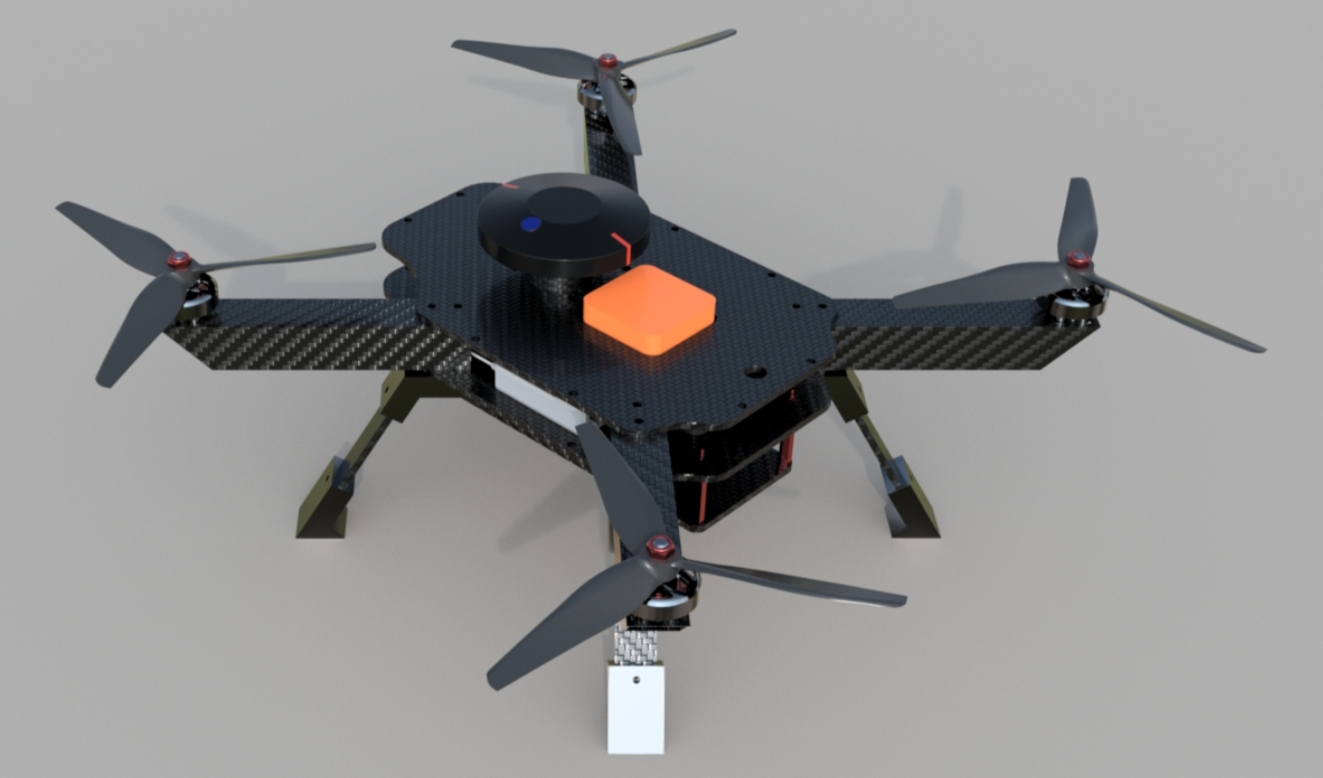
\includegraphics[scale=0.12]{render_drone.jpg}
            \caption{Rendered CAD Design}
            \label{fig: render_drone}
        \end{figure}

    \end{minipage}
    \begin{minipage}{0.47\textwidth}
        \vspace{0.2cm}
        \begin{figure}[h!]
            \centering
            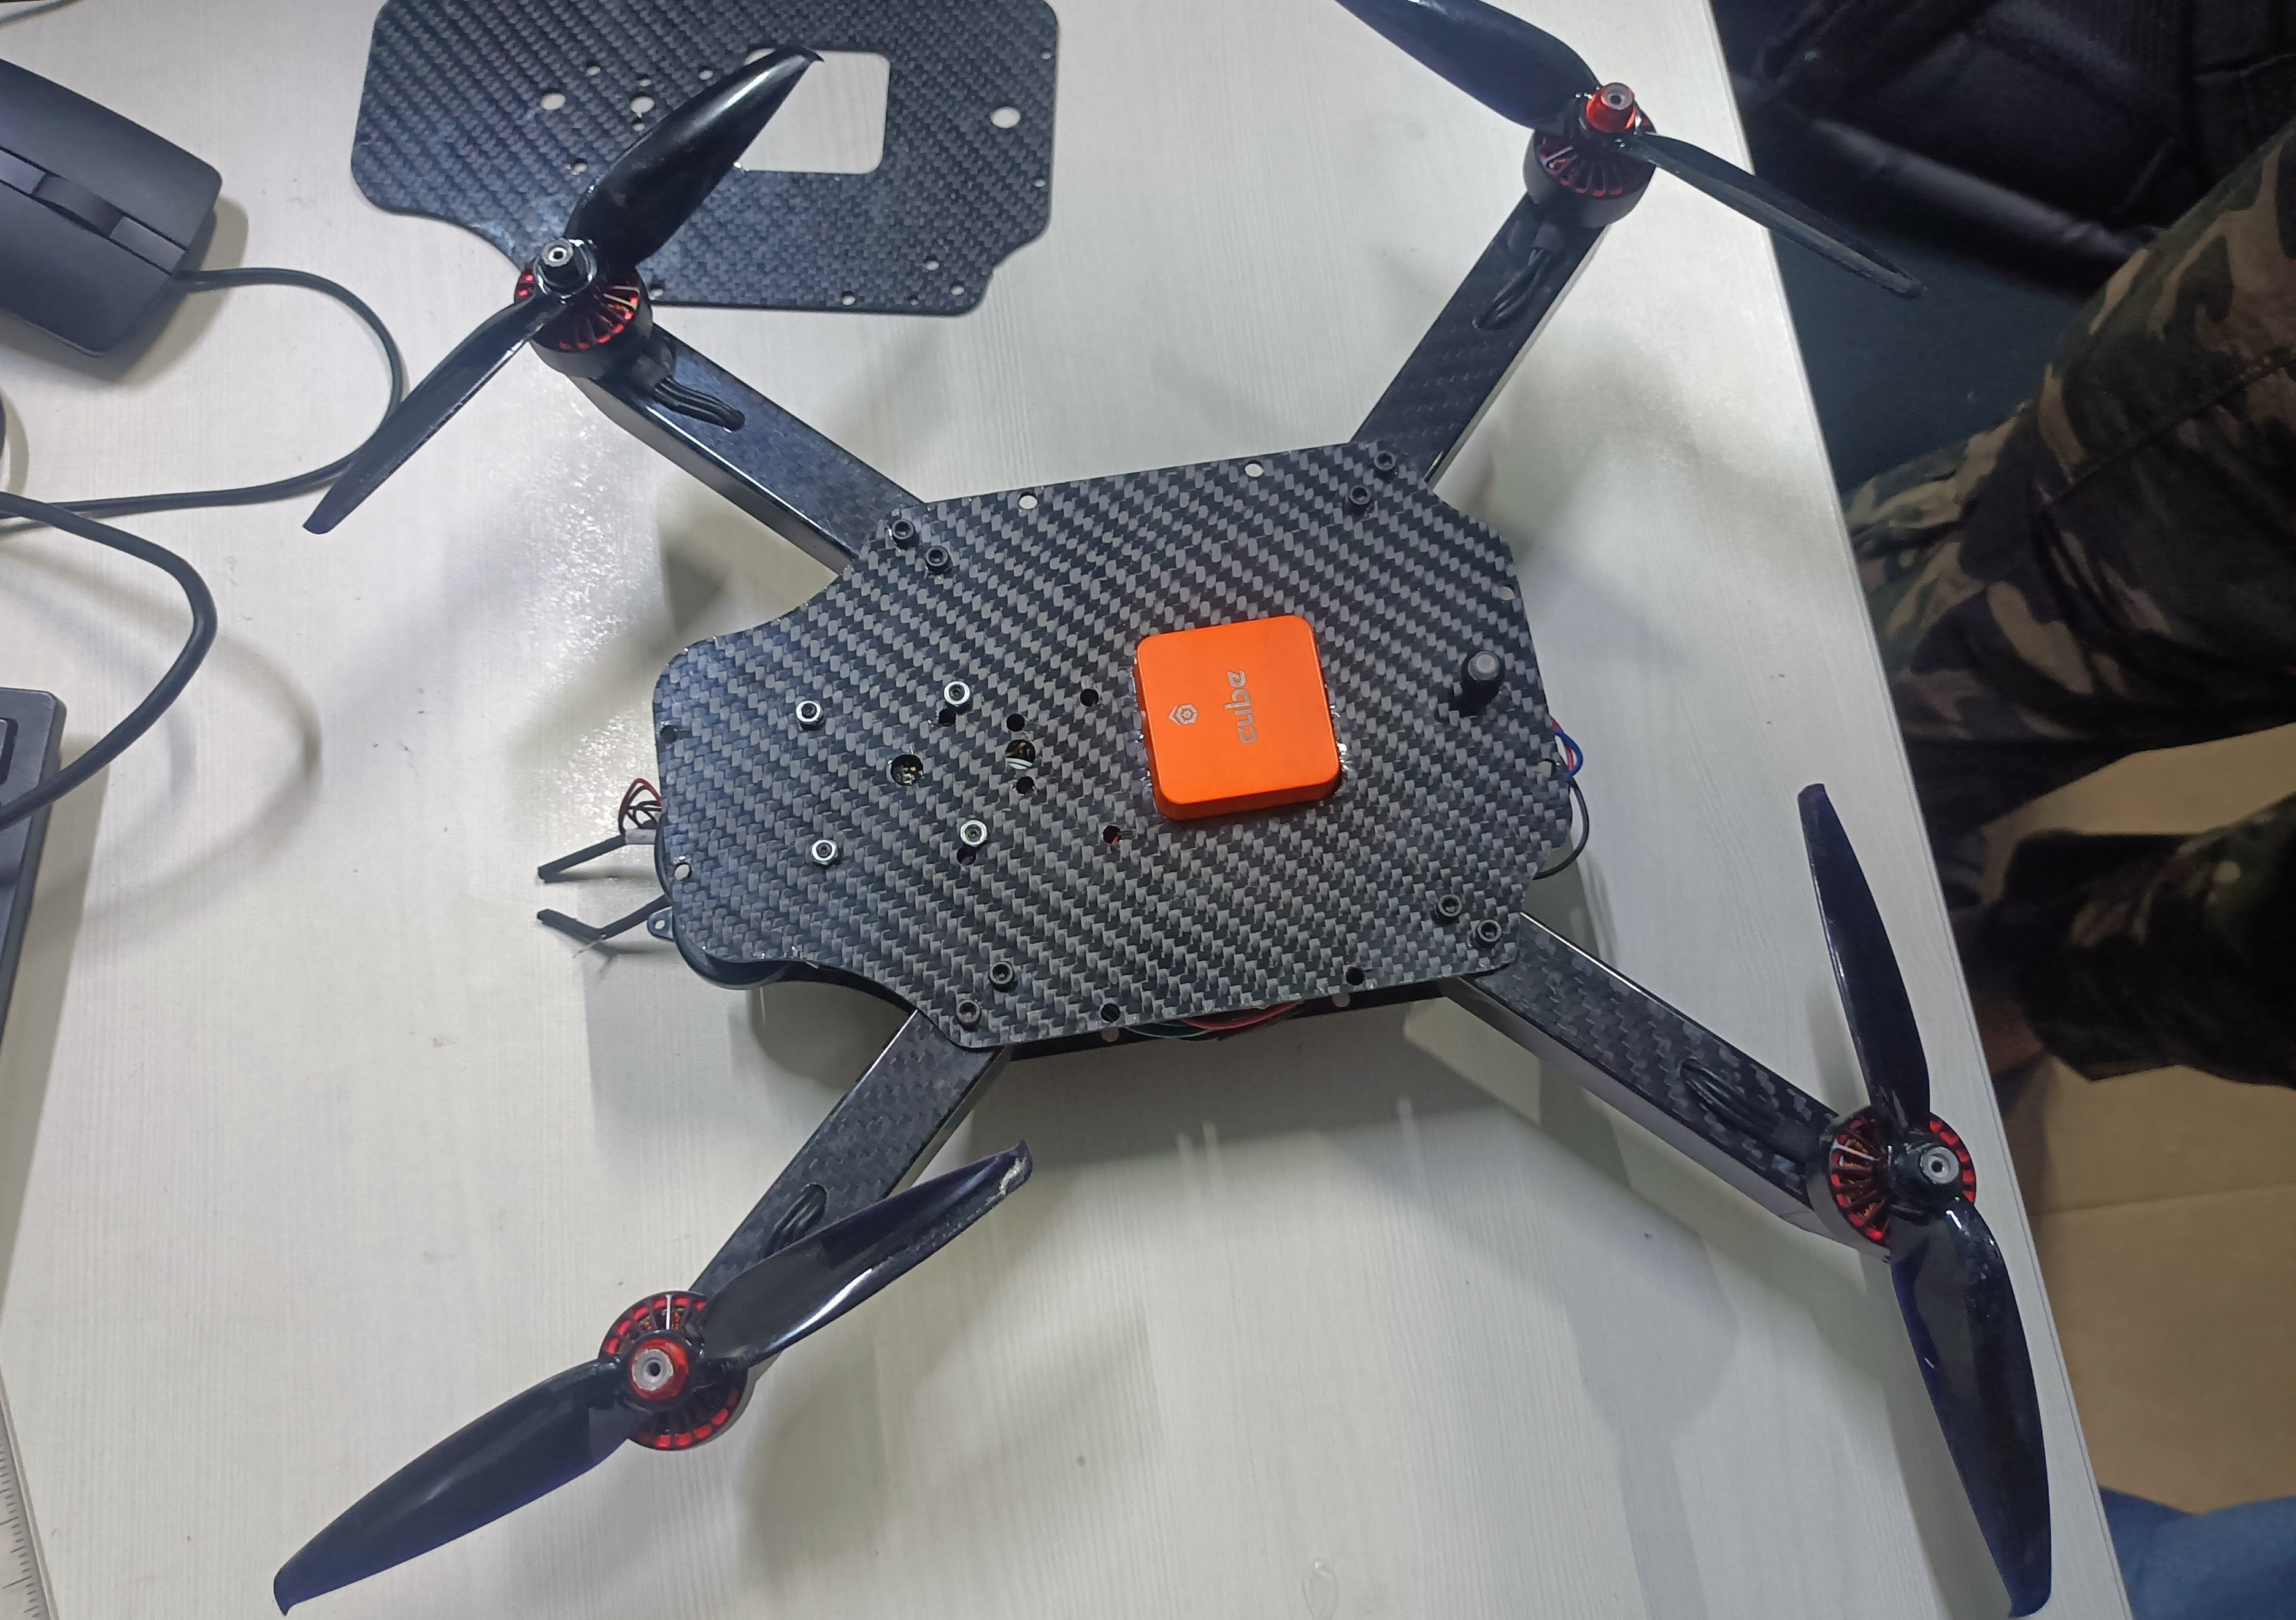
\includegraphics[scale=0.04]{real_drone.jpg}
            \caption{Real Developed drone}
            \label{fig: real_drone}
        \end{figure}

    \end{minipage}
\end{frame}


\subsection*{Experiments and Results}
\begin{frame}{Experiments and Results}
    \begin{description}
        \item[1. Thermal Camera Calibration]
    \end{description}{}

    \begin{figure}[h!]
        \centering
        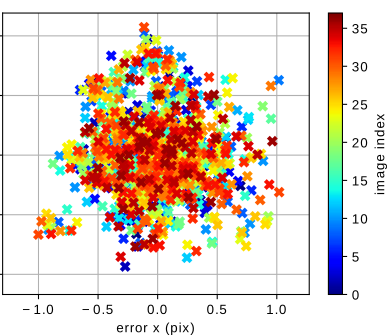
\includegraphics[scale=0.30]{Thermal_calibration.png}
        \caption{Reprojection Error}
        \label{fig: rej-error}
    \end{figure}
    \pause
    \vspace{-0.5cm}
        \begin{itemize}
            \item Intrinsic Camera Matrix \\ 
            \begin{equation*}
                \mathbf{K} = \begin{bmatrix}
                    414 & 0   & 340 \\
                    0   & 422 & 280 \\
                    0   & 0   & 1
                \end{bmatrix}
            \end{equation*}
            \pause
            
            \item Distortion parameters $\mathbf{(k1,k2,p1,p2)}=[-0.348,~  0.093,~ -0.011,~ -0.008]$
        \end{itemize}

\end{frame}

\begin{frame}{}
    \begin{description}
        \item[2. Thermal Odometry]
    \end{description}{}
    \begin{itemize}
        \item Thermal Odomery was performed on the dataset available online.
        \item The full video is \includemovie[
            poster,
            autoplay,
            externalviewer,
            inline=true,
            text={ i}
            ]{0.3cm}{0.3cm}{thermal_odometry.mp4} 
    \end{itemize}
    \begin{figure}[h!]
        \centering
        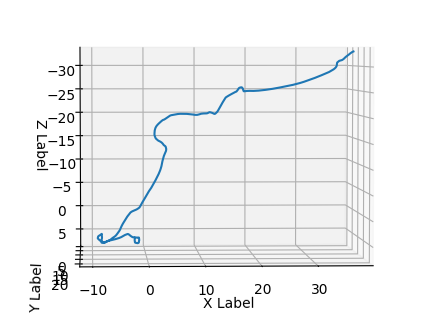
\includegraphics[scale=0.45]{Thermal_odometry.png} 
        \caption{Thermal Odometry}
        \label{Fig:thermal_odometry}
    \end{figure}
        
\end{frame}

\begin{frame}{}
    \begin{description}
        \item[3. Drone in Fire]
    \end{description}{}
    \begin{itemize}
        \item Pool fire of 0.8m was lited for the experiment.
        \item Drone was controlled in Althold mode using barometer data.
        \item No significant effect of soot and smoke on pressure readings.
        \item The full video is \includemovie[
            poster,
            autoplay,
            externalviewer,
            inline=true,
            text={ i}
            ]{0.3cm}{0.3cm}{flir.mp4} 
    \end{itemize}
    \begin{figure}[h!]
        \centering
        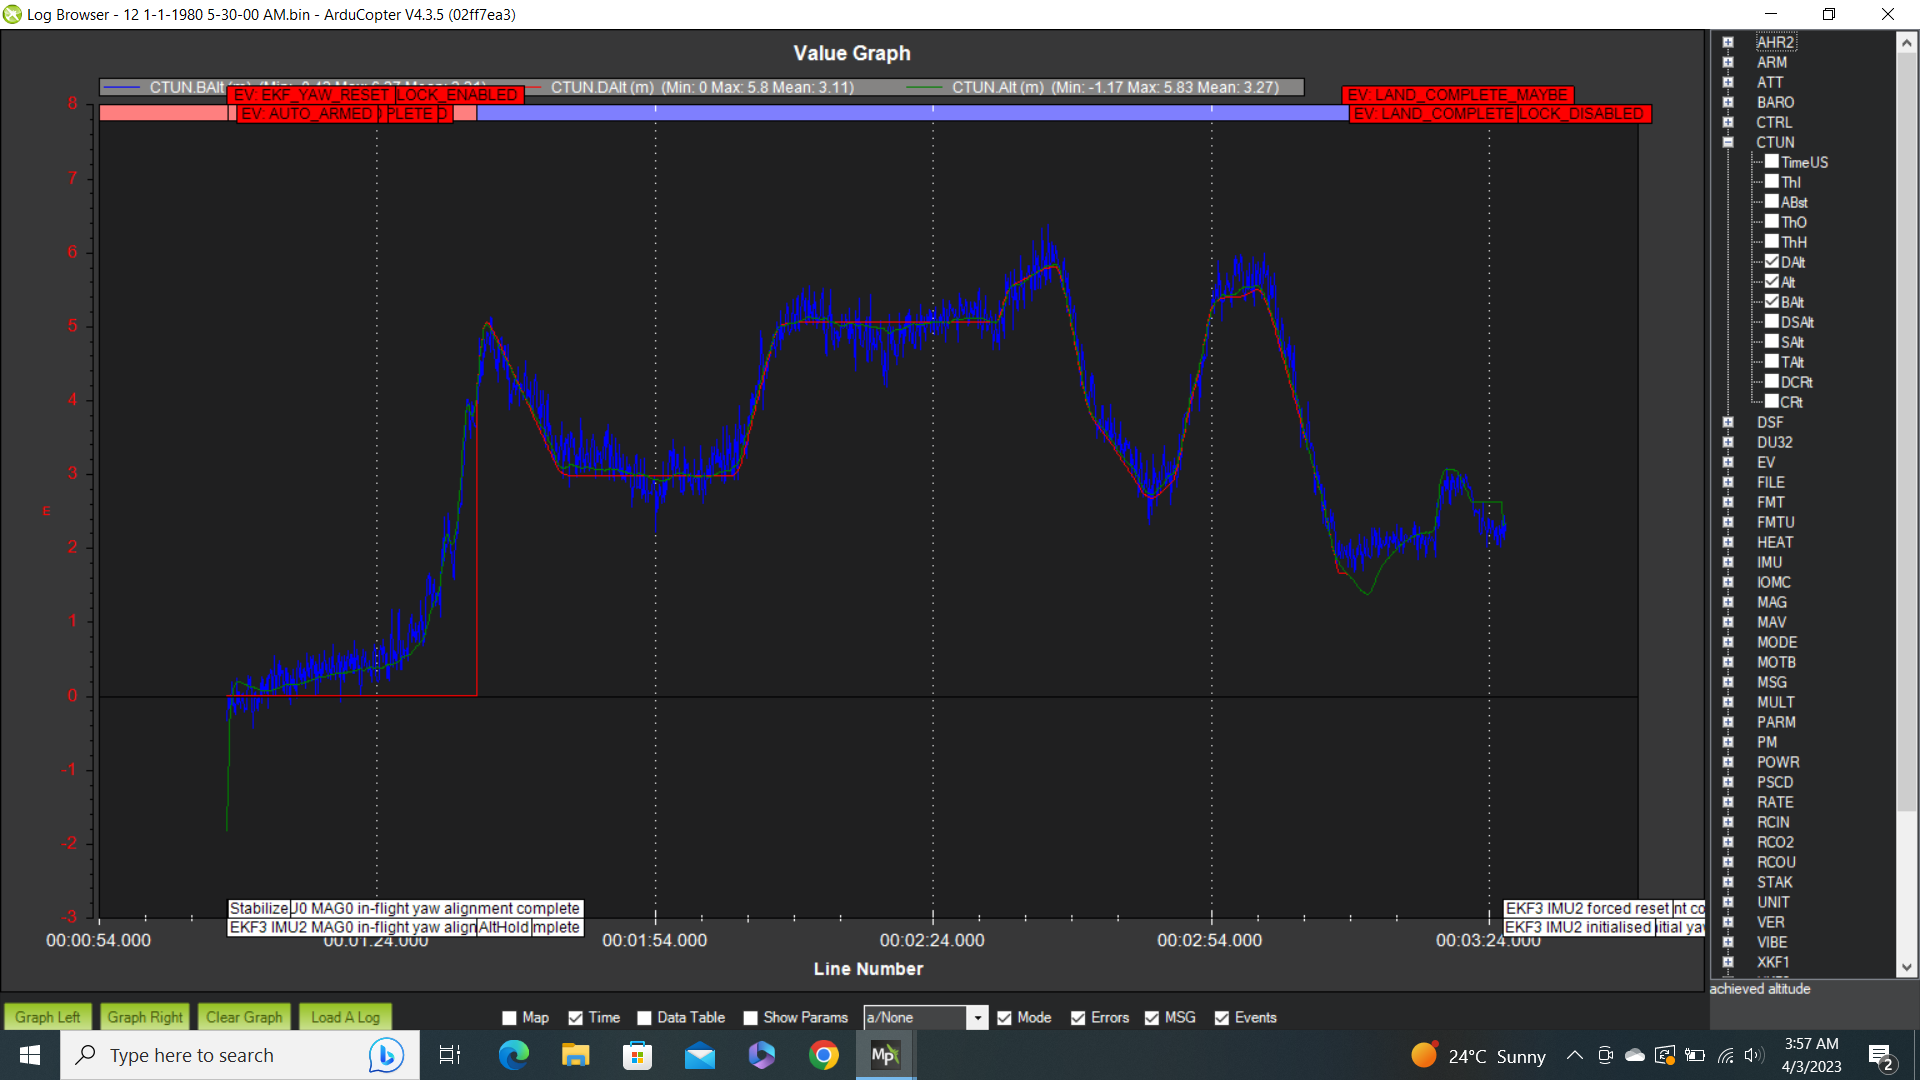
\includegraphics[scale=0.15]{uav_log.png} 
        \caption{Altitute hold data}
        \label{Fig:alt_data}
    \end{figure}

\end{frame}

\section*{}
\begin{frame}{}
    \huge{\centerline{\textcolor{blue}{\textbf{4. Multiagent System Simulation}}}}
\end{frame}
\section{Multiagent System Simulation Platform \textbf{MASCOT}}
\subsection*{Objective and System Architecture}
\begin{frame}{Objective and System Architecture}
\begin{itemize}
    \item Swarms in formation and rapid exploration.
    \item Rapid exploration of environment
\end{itemize}{}
    \begin{figure}[h!]
        \centering
        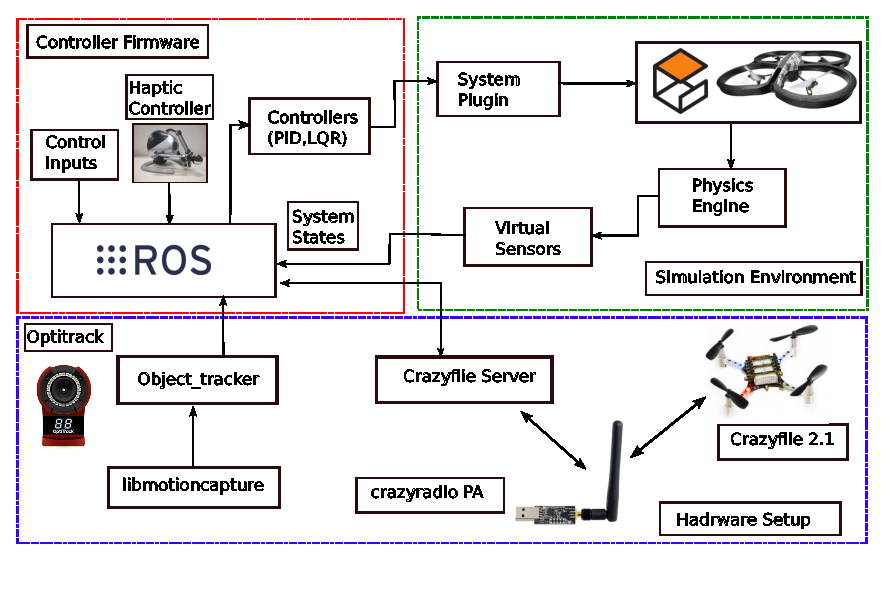
\includegraphics[scale=0.7]{System-architecture_final.eps} 
        \vspace{-0.3cm}
        \caption{System Architecture}
        \label{Fig:mas_system}
    \end{figure}

\end{frame}{}
\subsection*{Dynamics of Quadcopter}
\begin{frame}{Dynamics of Quadcopter}
    \begin{minipage}{0.47\textwidth}
    \begin{itemize}
         \item Total force on quadcopter 
            \begin{equation*}
            \mathbf{f}^{B^{\prime}}=\mathbf{R}{x}\left(\theta{r}\right) \mathbf{R}{y}\left(\theta{p}\right)\begin{bmatrix}
            0 & 0 & T
            \end{bmatrix}^{T}\label{eq:total_force}
            \end{equation*}

            \item Thus we get $\mathbf{f}^{B^{\prime}}$ as  
            \begin{equation*}
            \mathbf{f}^{B^{\prime}}=\begin{bmatrix}
            T\sin{\theta_{p}} \\
            T\sin{\theta_{r}}\cos{\theta_{p}} \\
            T\cos{\theta_{r}}\cos{\theta_{p}}
            \end{bmatrix}
            \end{equation*}
    \end{itemize}	
	\end{minipage}
	\begin{minipage}{0.47\textwidth}
             \begin{figure}[h!]
			\centering
			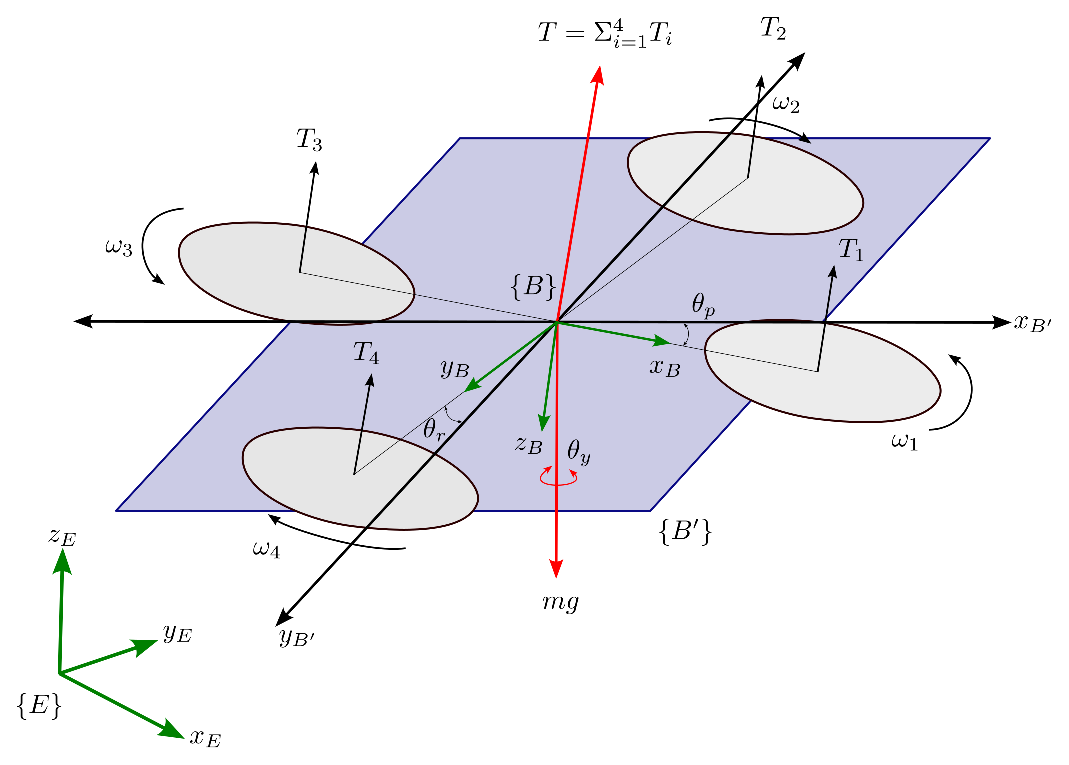
\includegraphics[scale=0.28]{Quadcopter.eps} 
			\caption{Quadcopter Dynamics}
			\label{Fig:Quadcopter Dynamics}
		\end{figure}
	\end{minipage}
        
 \begin{itemize}
    \item For small $\theta_{p}$ and $\theta_{r}$ the $\mathbf{f}^{B^{\prime}}$ can be approximated by 
\begin{equation*}
\mathbf{f}^{B^{\prime}} \approx \begin{bmatrix}
T\theta_{p} & T\theta_{r} & T
\end{bmatrix}^{T}
\end{equation*} 
    \item With this assumption the Quadcopter can be assumed as a double integrator system where $\theta_{p}$ and $\theta_{r}$ are given by
    \begin{equation*}
        \theta_{p} = \dfrac{m}{T}a_{x}^{B^{\prime}},~~\theta_{r} = \dfrac{m}{T}a_{y}^{B^{\prime}}
    \end{equation*}
    \end{itemize}
\end{frame}
\subsection*{Feature of Simulation Testbed}

\begin{frame}{Feature of Simulation Testbed}
    \begin{itemize}
        \item Easy Modification and support for HITL and Hybrid Hardware Simulation.
        \item Supports multiple languages Python, Cpp, Java
        \item Flexibility with no. of Agents 
    \end{itemize}
\begin{minipage}{0.47\textwidth}
    \begin{itemize}
    \item \textbf{Robot:} Details of the Robots to be simulated
        \begin{itemize}
            \item \textbf{Number:} No. of Agents 
            \item \textbf{IntialPosition:} Enable initial.
            \item \textbf{Position:} Initial Position.
            \item \textbf{Virtual:} Virtual or Real
        \end{itemize}	
    \item \textbf{Output:} Output config
        \begin{itemize}
            \item \textbf{Velocity : }Generate Vel plot
            \item \textbf{Position : }Generate Vel plot
            \item \textbf{Save-plot : }Save plots.
            \item \textbf{Show-plot : }Show plots
            \item \textbf{Save-data : }Save Numpy array
        \end{itemize}
\end{itemize}
\end{minipage}
\begin{minipage}{0.47\textwidth}
    \begin{itemize}
        \item \textbf{Control: }Controls laws
        \begin{itemize}
            \item \textbf{Custom-Control: }
            \item \textbf{Tutorial Examples: }
            \item[*] \textbf{Waypoint Navigation:}
            \begin{itemize}
                \item[-] \textbf{P-Gain: }Default = 1.0
                \item[-] \textbf{D-Gain: }Default = 1.0
            \end{itemize}
            \item[*] \textbf{Consensus: }
            \begin{itemize}
                \item[-] \textbf{Leader: }Robot index to be leader, 0-for leaderless consensus.
            \end{itemize}
            \item[*] \textbf{Min-max Consensus: }
            \item[*] \textbf{Formation: }
            \begin{itemize}
                \item[-] \textbf{Shape: }Square, Hexagon.
            \end{itemize}
        \end{itemize}
    \end{itemize}
\end{minipage}  
\end{frame}
\subsection*{Simulation Results}
\begin{frame}{Simulation Results}
    \begin{description}
        \item[1. Waypoint Navigation]
    \end{description}{}
\begin{minipage}{0.47\textwidth}
     \begin{figure}[h!]
			\centering
			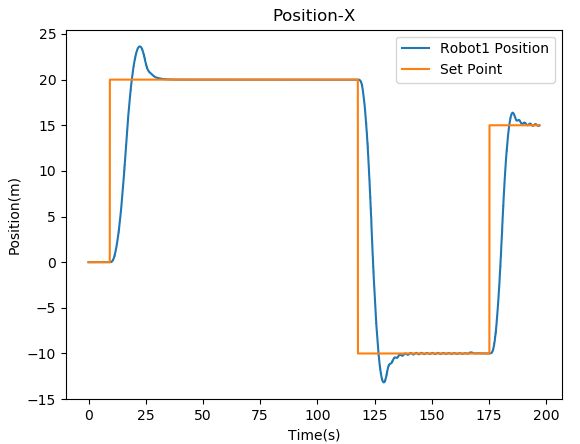
\includegraphics[scale=0.28]{Position-X-single.png} 
			\caption{X-axis Position plot }
			\label{Fig:pos_x}
		\end{figure}
	\end{minipage}
	\begin{minipage}{0.47\textwidth}
             \begin{figure}[h!]
			\centering
			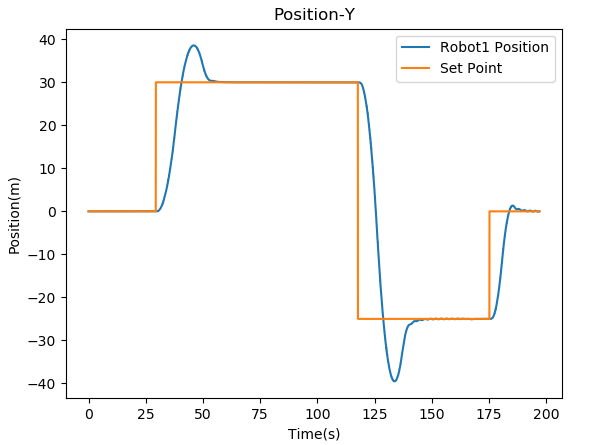
\includegraphics[scale=0.28]{Position-Y-single.png} 
			\caption{Y-axis Position plot }
			\label{Fig:pos_y}
		\end{figure}
	\end{minipage}

Part of this work is presented as:
\hspace{0.8cm}Arvind Pandit, Akash Njattuvetty, Ameer K. Mulla, ``ROS-Based \textbf{M}ulti-\textbf{A}gent \textbf{S}ystems \textbf{CO}ntrol Simulation \textbf{T}estbed (MASCOT)", in \textit{8th Indian Control Conference 2022}, Indian Institute of Technology Madras, India.(Presented)  
\end{frame}

\subsection*{Simulation Results}
\begin{frame}{}
    \begin{description}
        \item[2. Hybrid Formation Control]
    \end{description}{}
\begin{itemize}
    \item Hybrid Simulation in hexagon formation.
    \item Two crazyflies as real agent and 4 virtual agent.
    \item Haptic falcon is used for command controls.
    \item The full video is \includemovie[
        poster,
        autoplay,
        externalviewer,
        inline=true,
        text={ i}
        ]{0.3cm}{0.3cm}{hybrid.mp4} 
   \end{itemize}
   \begin{minipage}{0.47\textwidth}
    \begin{figure}[h!]
           \centering
           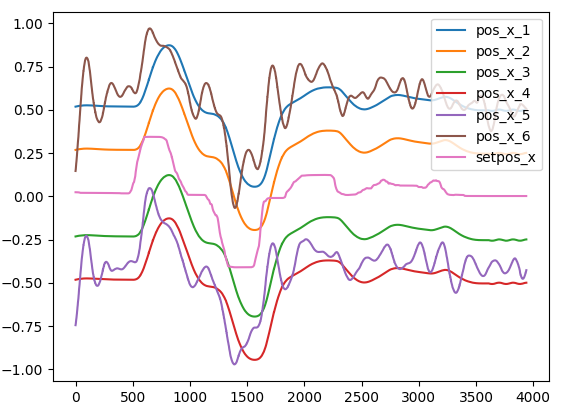
\includegraphics[scale=0.28]{hex_X.png} 
           \caption{Hexagaon Formation X-axis}
           \label{Fig:poshex_x}
       \end{figure}
   \end{minipage}
   \begin{minipage}{0.47\textwidth}
            \begin{figure}[h!]
           \centering
           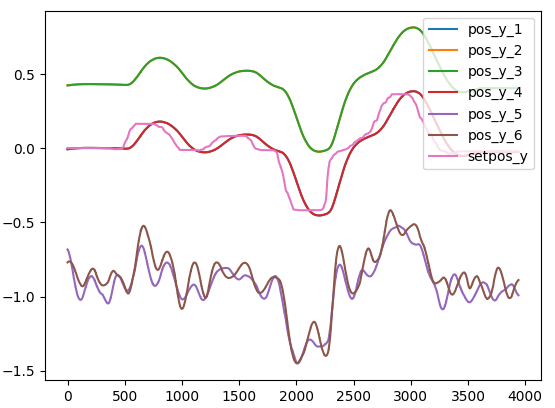
\includegraphics[scale=0.28]{hex_Y.png} 
           \caption{Hexagaon Formation Y-axis}
           \label{Fig:poshex_y}
       \end{figure}
   \end{minipage} 
\end{frame}

\section*{}
\begin{frame}{}
    \huge{\centerline{\textcolor{blue}{\textbf{5. Conclusion and Future Work}}}}
\end{frame}

\section{Conclusion and Future Work}
\begin{frame}{Conclusion and Future Work}
    \begin{block}{Conclusion}
        \begin{itemize}
            \item Developed a Visual Inertial Navigation system which uses only a monocular camera and IMU for navigation task.
            \item Camera calibration of LWIR camera and Thermal Odometry. 
            \item Drone design and testing.
            \item Multiagent System Simulation Platform.
        \end{itemize}
    \end{block}

    \pause \begin{block}{Future Work}
        \begin{itemize}
            \item Monocular VINS on quadcopter and navigation.
            \item Optimizing 3D reconstruction and dense mapping
            \item Path planning and exploration
            \item Navigation using Thermal Camera.
            \item Multivehicle hybrid Simulation for MASCOT.
        \end{itemize}
    \end{block}
\end{frame}



\section*{}
\begin{frame}{}
    \Huge{\centerline{\textcolor{blue}{\textbf{Thank You}}}}
\end{frame}
\end{document}